%%%%%%%%%%%%%%%%%%%%%%%%%%%%%%%%%%%%%%%%%%%%%%%%%%%%%%%%%%%%%%%%%%%
%%%%%%%%%%%%%%%%%%%%%%%%%%%%%%%%%%%%%%%%%%%%%%%%%%%%%%%%%%%%%%%%%%%
\chapter{Fundamentação Teórica} \label{cap:fund}
%%%%%%%%%%%%%%%%%%%%%%%%%%%%%%%%%%%%%%%%%%%%%%%%%%%%%%%%%%%%%%%%%%%
%%%%%%%%%%%%%%%%%%%%%%%%%%%%%%%%%%%%%%%%%%%%%%%%%%%%%%%%%%%%%%%%%%%
    
    Este capítulo tem como objetivo apresentar as teorias que embasam os conversores estáticos, desde os convencionais até a topologia utilizada nesse trabalho. Em seguida, um referencial teórico sobre compatibilidade eletromagnética, abordando os geradores e receptores de ruído, normas de EMC e técnicas para mitigação de ruído são apresentados. 
    
    %%%%%%%%%%%%%%%%%%%%%%%%%%%%%%%%%%%%%%%%%%%%%%%%%%%%%%%%%%%%%%%%%%%
    \section{Conversores estáticos} \label{cap:fund_elp}
    %%%%%%%%%%%%%%%%%%%%%%%%%%%%%%%%%%%%%%%%%%%%%%%%%%%%%%%%%%%%%%%%%%%
        
        Os circuitos eletrônicos de potência são dispositivos eletrônicos que convertem um tipo ou nível de tensão ou corrente para outro. Com suas aplicações variando de alguns watts até megawatts, de carregadores de celular até sistema de geração de energia eólica. Por converterem um tipo ou nível de uma forma de onda de tensão ou corrente em outro, são chamados de conversores. Os conversores, como apresentado na \autoref{fig:fonte_conv_carga}, servem como uma interface entre a fonte de energia e a carga \cite{ref:ELP_livro_Hart}.
        % sistemas de iluminação
        
        \begin{figure}[H]
        	\centering
        	\caption{Representação simplificada de um conversor}
        	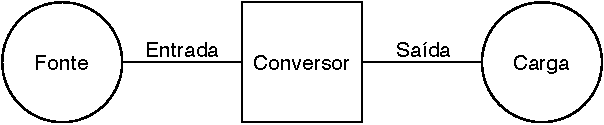
\includegraphics[scale=1]{pdf/outros/fonte_conver_carga.pdf}
        	\label{fig:fonte_conv_carga}
         	\indentedfont[10cm]{Adaptado de \citeonline[p.~2]{ref:ELP_livro_Hart}}
        \end{figure}
        
        \citeonline{ref:ELP_livro_Hart} afirma que os conversores podem ser classificados em quatro aplicações básicas: a conversão de \abreviatura*{CA}{corrente alternada} para \abreviatura*{CC}{corrente contínua}, também conhecidos como retificadores, a conversão de CC para CA, conhecidos como inversores, a conversão de determinado nível de tensão CC para outro nível de tensão CC e a conversão de uma fonte de energia CA com uma amplitude e frequência para amplitude e frequência diferentes. 
        % Neste trabalho será abordado apenas os conversores que convertem diferentes níveis de tensão CC, também conhecidos como conversores \mbox{CC-CC}.
        
        %%%%%%%%%%%%%%%%%%%%%%%%%%%%%%%%%%%%%%%%%%%%%%%%%%%%%%%%%%%%%%%%%%%
        \subsection{Conversor linear e chaveado} \label{cap:fund_elp_convlc}
        %%%%%%%%%%%%%%%%%%%%%%%%%%%%%%%%%%%%%%%%%%%%%%%%%%%%%%%%%%%%%%%%%%%
            
            Para \citeonline{ref:ELP_livro_Hart}, um método simples para a conversão de diferentes níveis de tensão CC consiste no uso de um circuito conhecido como conversor linear. O autor ainda apresenta a estrutura básica desse conversor como observado na \autoref{fig:conver_linear}.
            
            \begin{figure}[H]
            	\centering
            	\caption{Representação simplificada de um conversor CC-CC linear}
            	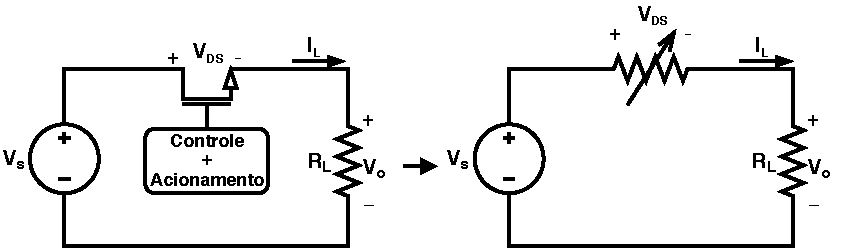
\includegraphics[scale=1]{pdf/outros/conver_linear.pdf}
            	\label{fig:conver_linear}
             	\indentedfont[14.5cm]{Adaptado de \citeonline[p.~197]{ref:ELP_livro_Hart}}
            \end{figure} 
            
            Nessa estrutura o transistor presente no circuito, operando na região de triodo, se comporta como uma resistência variável, controlando o valor da tensão de saída $\subx{V}{o}$, através da queda de tensão sobre ele. Assim, possibilitando que a tensão de saída seja regulada entre 0 e aproximadamente $\subx{V}{s}$ \cite{ref:ELP_livro_Hart}.
            
            Apesar de ser uma solução simples, \citeonline{ref:ELP_livro_Hart} adverte que a baixa eficiência desse circuito é uma desvantagem significante para aplicações de potência. Tal fato se dá devido as perdas presentes no transistor ser igual a $\subx{V}{DS} \cdot \subx{I}{L}$, assim, não sendo possível transferir toda a potência de entrada para a carga $\subx{R}{L}$. 
            
            Uma alternativa mais eficiente ao conversor linear é o conversor chaveado, também conhecido como conversor estático \cite{ref:ELP_livro_Hart}, mostrado de forma simplificada na \autoref{fig:conver_chaveado}. 
            
            \begin{figure}[H]
            	\centering
            	\caption{Representação simplificada de um conversor CC-CC chaveado}
            	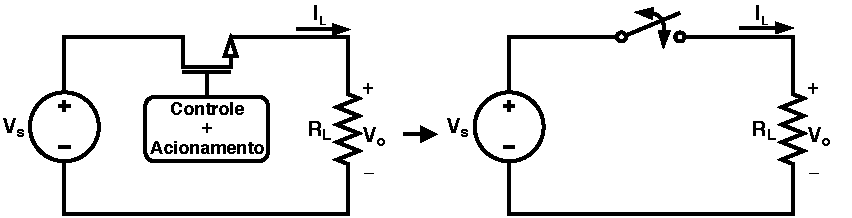
\includegraphics[scale=1]{pdf/outros/conver_chaveado.pdf}
            	\label{fig:conver_chaveado}
             	\indentedfont[14.5cm]{Adaptado de \citeonline[p.~197]{ref:ELP_livro_Hart}}
            \end{figure}
            
            Nesse circuito, o transistor opera como uma chave eletrônica, sendo completamente ligado ou desligado. Assim, tendo como base o circuito da \autoref{fig:conver_chaveado}, a abertura e o fechamento periódico da chave resultam na tensão de saída $\subx{V}{o}$ observada na \autoref{fig:conver_chaveado_onda}.
            
            \begin{figure}[H]
            	\centering
            	\caption{Tensão de saída de um conversor CC-CC chaveado simples}
            	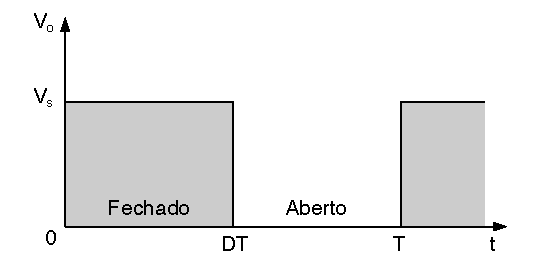
\includegraphics[scale=1]{pdf/outros/tensao_conver_chaveado.pdf}
            	\label{fig:conver_chaveado_onda}
             	\indentedfont[8cm]{Adaptado de \citeonline[p.~197]{ref:ELP_livro_Hart}}
            \end{figure}
            
            Para \citeonline{ref:ELP_livro_Hart}, o valor médio dessa tensão de saída pode ser obtida através da \autoref{eq:conver_chav_Vo_medio}, sendo a razão cíclica D igual a divisão entre o tempo da chave fechada pelo período total T.
            
            \begin{equation} \label{eq:conver_chav_Vo_medio}
                \subx{V}{o\_med} = \frac{1}{\text{T}} \int_{0}^{T} \subx{V}{s}\cdot\text{dt} = \subx{V}{s}\cdot\text{D}
            \end{equation}
            
            \begin{conditions}
                \subx{V}{o\_med}     & Valor médio da tensão de saída (V)\\
                \text{T}            & Período de comutação (s) \\
                \subx{V}{s}         & Tensão de entrada (V) \\
                \text{D}            & Razão cíclica 
            \end{conditions}
            
            Assim, o valor médio da tensão de saída $\subx{V}{o\_med}$ pode ser controlada ajustando a razão cíclica D, podendo ser igual ou inferior a tensão de entrada $\subx{V}{s}$ do circuito. 
            
            \citeonline{ref:ELP_livro_Hart} afirma que, considerando a chave como sendo ideal, a potência dissipada por ela será igual a zero. Pois, estando a chave aberta, não haverá corrente circulando no circuito e quando a chave estiver fechada, a tensão sobre ela é nula. Portanto, toda a potência é absorvida pela carga e a eficiência energética do circuito é de 100\%. Porém, em um circuito real ocorrerão perdas, uma vez que a tensão sobre a chave fechada não é zero e a chave apresenta tempos diferentes de zero para realizar a comutação entre fechada para aberta ou vice-versa. 
            
            %%%%%%%%%%%%%%%%%%%%%%%%%%%%%%%%%%%%%%%%%%%%%%%%%%%%%%%%%%%%%%%%%%%
            \subsubsection{Conversor estático do tipo Buck} \label{cap:fund_elp_convlc_convest}
            %%%%%%%%%%%%%%%%%%%%%%%%%%%%%%%%%%%%%%%%%%%%%%%%%%%%%%%%%%%%%%%%%%%
            
            Para \citeonline{ref:ELP_livro_Hart}, apesar do circuito presente na \autoref{fig:conver_chaveado} possuir uma componente CC controlável com uma tensão pulsada na saída, podendo ser suficiente para algumas aplicações, muitas vezes é necessário que essa tensão de saída seja puramente CC. Uma maneira de se obter essa saída é fazendo uso do circuito juntamente de um filtro passa-baixa. Essa estrutura, mostrada na \autoref{fig:conver_buck_simples}, é chamada de conversor Buck ou conversor abaixador, devido à tensão de saída ser menor que a de entrada. 
            
            \begin{figure}[H]
            	\centering
            	\caption{Estrutura básica de um conversor Buck}	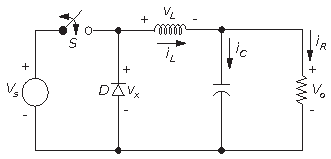
\includegraphics[scale=1.5]{pdf/outros/conversor_buck.pdf}
            	\label{fig:conver_buck_simples}
             	\indentedfont[8.7cm]{Adaptado de \citeonline[p.~199]{ref:ELP_livro_Hart}}
            \end{figure}
            
            \begin{conditions}
                \subx{i}{C}     & Corrente sobre o capacitor (A) \\
                \subx{i}{L}     & Corrente sobre o indutor (A) \\
                \subx{i}{R}     & Corrente sobre o resistor (A) \\
                \subx{V}{L}     & Tensão sobre o indutor (V)\\
                \subx{V}{o}     & Tensão de saída do circuito (V)\\
                \subx{V}{s}     & Tensão de entrada do circuito (V)\\
                \subx{V}{x}     & Tensão sobre o diodo (V) 
            \end{conditions}
            
            O diodo D adicionado a estrutura fornece um caminho para a corrente do indutor quando a chave S está aberta e sofre polarização reversa quando a chave S está fechada. A tensão $\subx{V}{x}$ de entrada do filtro passa-baixa permanece semelhante a apresentada na \autoref{fig:conver_chaveado_onda}. $\subx{V}{x}$ será igual a $\subx{V}{s}$ quando a chave S estiver fechada e zero quando estiver aberta, desde que o diodo D permaneça polarizado diretamente e conduzindo \cite{ref:ELP_livro_Rashid}.
            
            Segundo \citeonline{ref:ELP_livro_ConversNIsolado}, este modo de operação em que a corrente no indutor se mantém positiva enquanto o circuito está em operação, como na \autoref{fig:conver_buck_ccm}, é denominado \abreviatura&{CCM}{Continuous conduction mode}{modo de condução contínua}. Porém, no caso em que a corrente do indutor retorna a zero (\autoref{fig:conver_buck_dcm}), é denominado \abreviatura&{DCM}{Discontinuous conduction mode}{modo de condução descontínua}. 
            
            \begin{figure}[H]
                \centering
                \caption{Corrente no indutor para diferentes modos de operação do conversor}
                \begin{subfigure}[H]{.49\textwidth}
                    \centering
                    \caption{Modo de condução contínua}
                    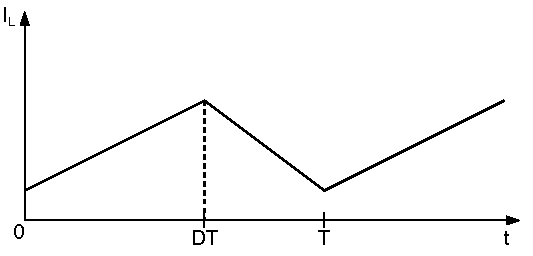
\includegraphics[scale=.85]{pdf/outros/CCM.pdf}
                    \label{fig:conver_buck_ccm}
                \end{subfigure}
                \begin{subfigure}[H]{.49\textwidth}
                    \centering
                    \caption{Modo de condução descontínua}
                    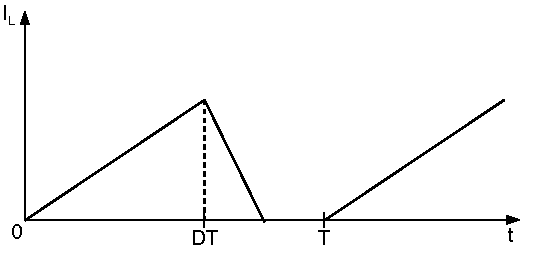
\includegraphics[scale=.85]{pdf/outros/DCM.pdf}
                    \label{fig:conver_buck_dcm}
                \end{subfigure}
                \indentedfont[15.5cm]{Elaboração própria (2021)}
            	\label{fig:conver_buck_ccm_dcm}
            \end{figure}
            
            Cada modo de operação possui suas características, vantagens e desvantagens. Dentre as características do CCM, pode-se citar que o ganho de tensão da estrutura não depende da carga, a ondulação de corrente no indutor é menor que a componente média e a estrutura apresenta maior eficiência energética em comparação com o DCM \cite{ref:ELP_livro_ConversNIsolado}. 
            
            No DCM, o seu ganho de tensão depende dos parâmetros da carga e dos componentes de filtro (indutor e capacitor), a ondulação de corrente e corrente eficaz do indutor é maior e o tamanho do indutor pode ser consideravelmente reduzido em comparação com o CCM \cite{ref:ELP_livro_ConversNIsolado}. 
            
            Assim, dadas essas características, neste trabalho optou-se por abordar apenas o projeto de filtros de conversores operando no modo de condução contínua.
            
            %%%%%%%%%%%%%%%%%%%%%%%%%%%%%%%%%%%%%%%%%%%%%%%%%%%%%%%%%%%%%%%%%%%
            \subsubsection{Modo de condução contínua} \label{cap:fund_elp_convlc_ccm}
            %%%%%%%%%%%%%%%%%%%%%%%%%%%%%%%%%%%%%%%%%%%%%%%%%%%%%%%%%%%%%%%%%%%
            
            No modo de condução contínua, com o objetivo de facilitar a compreensão, o circuito do conversor estático do tipo Buck será dividido em duas etapas de funcionamento. A \autoref{fig:conver_buck_simples_ab} apresenta as etapas de operação desse circuito \cite{ref:ELP_livro_Hart}.
            
            \begin{figure}[H]
                \centering
                \caption{Etapas de funcionamento do conversor estático do tipo Buck}
                \begin{subfigure}[H]{.49\textwidth}
                    \centering
                    \caption{Etapa 1: Chave fechada}
                    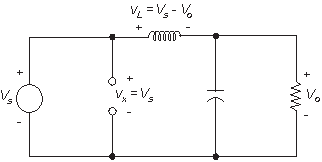
\includegraphics[scale=1.4]{pdf/outros/conversor_buck_desc_a.pdf}
                    \label{fig:conver_buck_simples_a}
                \end{subfigure}
                \begin{subfigure}[H]{.49\textwidth}
                    \centering
                    \caption{Etapa 2: Chave aberta}
                    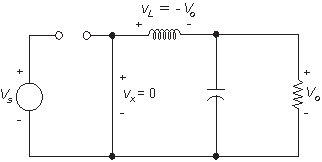
\includegraphics[scale=1.4]{pdf/outros/conversor_buck_desc_b.pdf}
                    \label{fig:conver_buck_simples_b}
                \end{subfigure}
                \indentedfont[15.5cm]{Adaptado de \citeonline[p.~199]{ref:ELP_livro_Hart}}
            	\label{fig:conver_buck_simples_ab}
            \end{figure}
            
            Na primeira etapa (de 0 a DT), observada na \autoref{fig:conver_buck_simples_a}, o transistor entra em condução e o diodo não conduz por estar polarizado reversamente. Portanto, a corrente de entrada do circuito circula pelo indutor e é distribuída entre o capacitor e a carga. Nesse processo, a fonte de tensão da entrada fornece energia elétrica para a saída e para a magnetização do indutor, assim, a corrente que circula no indutor cresce, devido a tensão $\subx{V}{s} - \subx{V}{o}$ imposta sobre ele \cite{ref:ELP_livro_Hart}.
            
            A segunda etapa (de DT até T) ocorre quando o transistor para de conduzir e o diodo entra em condução por estar diretamente polarizado, como na \autoref{fig:conver_buck_simples_b}. Nessa etapa, a energia armazenada no indutor na forma de magnetização passa a fornecer a energia necessária para a carga, desmagnetizando-o e fazendo essa corrente decrescer constantemente até que o transistor volte a conduzir, retornando à primeira etapa \cite{ref:ELP_livro_Hart}. 
            
            Durante o processo de funcionamento do circuito, a componente CA da corrente no indutor é direcionada ao capacitor, enquanto a componente CC é enviada para a carga \cite{ref:ELP_livro_Hart}. A \autoref{fig:conver_buck_basico_onda} apresenta as principais formas de onda do circuito, onde pode ser observado a corrente $\subx{i}{L}$ e tensão $\subx{V}{L}$ sobre o indutor e a corrente $\subx{i}{C}$ no capacitor. 
            
            \begin{figure}[H]
            	\centering
            	\caption{Principais formas de onda do conversor estático Buck em MCC}
            	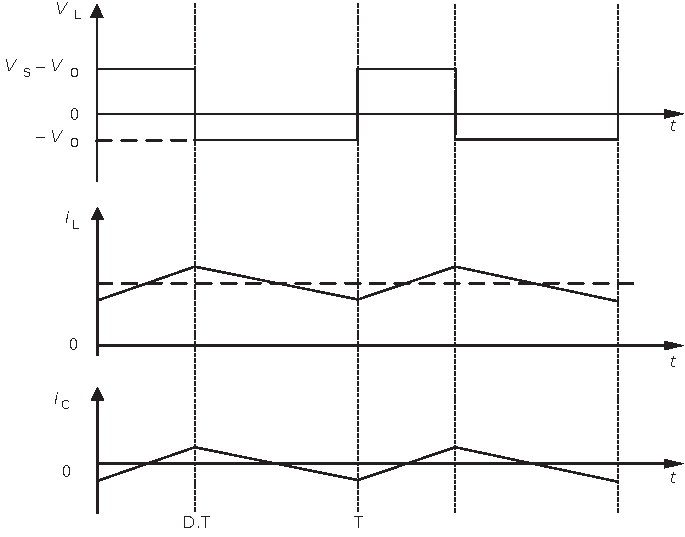
\includegraphics[scale=1.1]{pdf/outros/conversor_buck_forma_onda.pdf}
            	\label{fig:conver_buck_basico_onda}
             	\indentedfont[11.6cm]{Adaptado de \citeonline[p.~277]{ref:ELP_livro_Rashid}}
            \end{figure}
            
            Para que o conversor esteja operando em CCM, é necessário que a energia acumulada no indutor de 0 a D$\cdot$T seja igual a energia fornecida de D$\cdot$T a T. Assim, pode-se obter o valor da indutância L do filtro passa-baixa através da equação da tensão sobre o indutor, do período de 0 a D$\cdot$T, apresentado na \autoref{eq:buck_indutor} \cite{ref:ELP_livro_Hart}.
            
            \begin{equation} \label{eq:buck_indutor}
                \text{L} = 
                \frac{(\subx{V}{s} - \subx{V}{o})\cdot\text{D}}
                {\text{f}\cdot\Delta\subx{I}{L}}
            \end{equation}
            
            \begin{conditions}
                \text{D}            & Razão cíclica \\
                \text{f}            & Frequência de comutação do transistor (Hz) \\
                \Delta\subx{I}{L}   & Variação da corrente no indutor (A) \\
                \text{L}            & Indutância (H) \\
                \subx{V}{o}         & Tensão de saída do conversor (V) \\
                \subx{V}{s}         & Tensão de entrada do conversor (V) 
            \end{conditions}
            
            \citeonline{ref:ELP_livro_Hart} afirma que enquanto a corrente no capacitor for positiva, o capacitor estará carregando. Portanto, pela definição de capacitância, pode-se obter o seu valor através da equação de carga do capacitor. A \autoref{eq:buck_capacitor} apresenta a equação para o cálculo dessa capacitância.
            
            \begin{equation} \label{eq:buck_capacitor}
                \text{C} =
                \frac{\Delta\subx{I}{L}}
                {8\cdot\text{f}\cdot\Delta\subx{V}{o}}
            \end{equation}
            
            \begin{conditions}
                \text{C}            & Capacitância (F) \\
                \text{f}            & Frequência de comutação do transistor (Hz) \\
                \Delta\subx{I}{L}   & Variação da corrente no indutor (A) \\
                \Delta\subx{V}{o}   & Variação da tensão de saída do conversor (V)
            \end{conditions}
            
            Assim, obtêm-se as duas principais equações para projeto de um conversor estático do tipo Buck, totalmente dependentes de alguns parâmetros de projeto, como a variação de corrente no indutor $\Delta\subx{I}{L}$ e a variação de tensão na carga $\Delta\subx{V}{o}$. Ainda, nota-se pelas equações, que a escolha da frequência de comutação é de grande importância, uma vez que o seu aumento causa uma redução nos valores de indutância e capacitância e, consequentemente, uma redução no dimensionamento físico desses componentes. Por outro lado, aumenta as perdas nos elementos magnéticos e semicondutores \cite{ref:ELP_livro_Hart}. 
            
            %%%%%%%%%%%%%%%%%%%%%%%%%%%%%%%%%%%%%%%%%%%%%%%%%%%%%%%%%%%%%%%%%%%
            \subsubsection{Perdas por comutação e condução} \label{cap:fund_elp_convlc_perda}
            %%%%%%%%%%%%%%%%%%%%%%%%%%%%%%%%%%%%%%%%%%%%%%%%%%%%%%%%%%%%%%%%%%%
            
            Como mencionado na \autoref{cap:fund_elp_convlc}, para o caso em que os elementos semicondutores, transistor e diodo, forem ideais, o conversor não apresenta perdas de potência. Porém, ao utilizar componentes reais, algumas perdas devem ser consideradas. Essas perdas são necessárias para que seja possível dimensionar os componentes do circuíto e obter o rendimento do conversor \cite{ref:ELP_livro_ProjFontChav}. 
            
            Segundo \citeonline{ref:ELP_livro_ProjFontChav}, as perdas no diodo podem ser divididas em perdas por comutação e perdas por condução. Em condução, o diodo pode ser representado por uma força-eletromotriz $\subx{V}{(TO)}$ associada em série com uma resistência $\subx{r}{T}$. Essa equivalência é representada na \autoref{fig:equival_diodo}.
            
            \begin{figure}[H]
            	\centering
            	\caption{Representação da queda de tensão do diodo real e sua resistência interna}
            	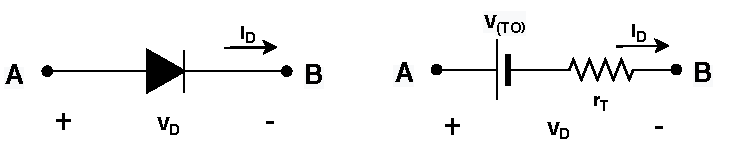
\includegraphics[scale=1]{pdf/perdas/modelo_diodo.pdf}
            	\label{fig:equival_diodo}
             	\indentedfont[12.5cm]{Elaboração própria (2021)}
            \end{figure}
            
            \begin{conditions}
                \subx{I}{D}             & Corrente no diodo (A) \\
                \subx{r}{T}             & Resistência série equivalente do diodo (\ohm) \\
                \subx{V}{D}             & Tensão direta no diodo (V) \\
                \subx{V}{(TO)}          & Tensão limiar de condução do diodo (V) 
            \end{conditions}
            
            Assim, as perdas por condução no diodo real podem ser obtidas através da \autoref{eq:perda_cond_diodo}.
            
            \begin{equation} \label{eq:perda_cond_diodo}
                \subx{P}{Dcond} = 
                \subx{V}{(TO)}\cdot\subx{I}{Dmed} + \subx{r}{T}\cdot\subx{I}{Drms}^2
            \end{equation}
            
            \begin{conditions}
                \subx{I}{Dmed}          & Valor da corrente média (A) \\
                \subx{I}{Drms}          & Valor da corrente eficaz (A) \\
                \subx{P}{Dcond}         & Perdas por condução no diodo (W) \\
                \subx{r}{T}             & Resistência série equivalente do diodo (\ohm) \\
                \subx{V}{(TO)}          & Tensão limiar de condução do diodo (V) 
            \end{conditions}
            
            Para a comutação, deve-se adicionar outro elemento a não idealidade do diodo, uma capacitância em paralelo $\subx{C}{D}$ (\autoref{fig:equival_diodo_cd}). Na fase de bloqueio do diodo, quando o transistor passa a conduzir, a corrente direta $\subx{I}{D}$ no diodo começa a decrescer, a uma taxa de velocidade dependente de $\subx{V}{s}$ e L \cite{ref:ELP_livro_EletrPotBarbi}. 
            
            \begin{figure}[H]
            	\centering
            	\caption{Representação da queda de tensão do diodo real, sua resistência e capacitância interna}
            	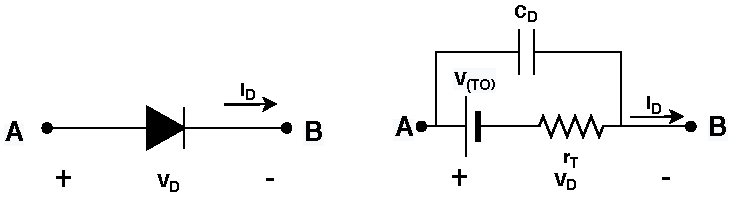
\includegraphics[scale=1]{pdf/perdas/modelo_diodo_CD.pdf}
            	\label{fig:equival_diodo_cd}
             	\indentedfont[12.5cm]{Elaboração própria (2021)}
            \end{figure}
            
            Após essa corrente ser nula, ocorre a descarga do capacitor $\subx{C}{D}$. Assim, a corrente $\subx{I}{D}$ torna-se negativa, durante um tempo $\subx{t}{rr}$ de recuperação reversa do diodo, até que a carga $\subx{Q}{rr}$ desse capacitor seja totalmente removida. Quando a carga $\subx{Q}{rr}$ se anula, o diodo se bloqueia. Com isso, o indutor L do circuito provoca uma sobretensão no diodo, podendo ser destrutivo para o mesmo \cite{ref:ELP_livro_EletrPotBarbi}. Essa sobretensão será melhor discutida na \autoref{cap:fund_emc}. Na \autoref{fig:perdas_diodo_c2} é  observado essas formas de onda.
            
            \begin{figure}[H]
            	\centering
            	\caption{Tensão e corrente em um diodo durante o bloqueio}
            	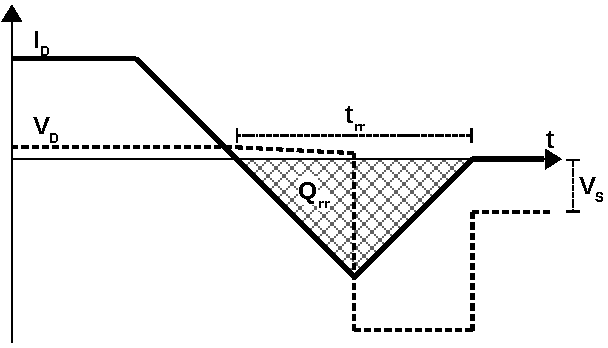
\includegraphics[scale=1]{pdf/perdas/perdas_diodo_c2.pdf}
            	\label{fig:perdas_diodo_c2}
             	\indentedfont[10.8cm]{Adaptado de \citeonline[p.~6]{ref:ELP_livro_EletrPotBarbi}}
            \end{figure}
            
            Assim, de acordo com \citeonline{ref:ELP_livro_EletrPotBarbi}, a \autoref{eq:perda_com1_diodo} apresenta as perdas provenientes da entrada em bloqueio do diodo. 
            
            \begin{equation} \label{eq:perda_com1_diodo}
                \subx{P}{1Dcom} = \subx{Q}{rr}\cdot\subx{V}{s}\cdot\text{f}
            \end{equation}
            
            \begin{conditions}
                \text{f}            & Frequência de comutação da chave (Hz) \\
                \subx{P}{1Dcom}     & Perdas por comutação no bloqueio do diodo (W) \\
                \subx{Q}{rr}        & Carga do capacitor intrínseco do diodo (C) \\
                \subx{V}{s}         & Tensão de entrada do conversor (V) 
            \end{conditions}
            
            Ainda, deve-se considerar a fase de entrada em condução do diodo, \autoref{fig:perdas_diodo_c1}, que, diferente do diodo ideal, leva um certo período de tempo $\subx{t}{rf}$ para entrar em condução \cite{ref:ELP_livro_EletrPotBarbi}. 
            %Segundo \citeonline{ref:ELP_livro_EletrPotBarbi}, esse tempo pode variar de \SI{0,1}{\micro\second} a \SI{1,5}{\micro\second}.
            
            \begin{figure}[H]
            	\centering
            	\caption{Formas de onda relativas à entrada em condução de um diodo}
            	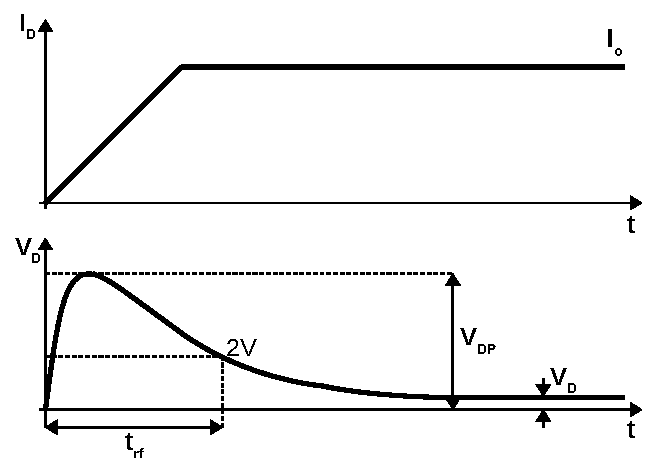
\includegraphics[scale=1]{pdf/perdas/perdas_diodo_c1.pdf}
            	\label{fig:perdas_diodo_c1}
             	\indentedfont[11cm]{Adaptado de \citeonline[p.~8]{ref:ELP_livro_EletrPotBarbi}}
            \end{figure}
            
            Como observado, nesse período $\subx{t}{rf}$, surge uma sobretensão $\subx{V}{DP}$ sobre esse diodo. Segundo \citeonline{ref:ELP_livro_EletrPotBarbi}, a \autoref{eq:perda_com2_diodo} apresenta as perdas no diodo proveniente da entrada em condução. 
            
            \begin{equation} \label{eq:perda_com2_diodo}
                \subx{P}{2Dcom} = 
                0,5\cdot(\subx{V}{DP} - \subx{V}{D})\cdot\subx{I}{o}\cdot\subx{t}{rf}\cdot\text{f}
            \end{equation}
            
            \begin{conditions}
                \text{f}            & Frequência de comutação da chave (Hz) \\
                \subx{I}{o}         & Corrente do diodo em condução (A) \\
                \subx{P}{2Dcom}     & Perdas por comutação na entrada em condução do diodo (W) \\
                \subx{t}{rf}        & Tempo de atraso na transição (s) \\
                \subx{V}{D}         & Tensão do diodo em condução (V) \\
                \subx{V}{DP}        & Tensão de pico do diodo na entrada em condução (V)
            \end{conditions}
            
            Assim, pode ser definido as perdas totais de comutação do diodo como sendo a soma de $\subx{P}{1Dcom} + \subx{P}{2Dcom}$, mostrado na \autoref{eq:perda_com_diodo} \cite{ref:ELP_livro_EletrPotBarbi}.
            
            \begin{equation} \label{eq:perda_com_diodo}
                \subx{P}{Dcom} = 
                0,5\cdot(\subx{V}{DP} - \subx{V}{D})\cdot\subx{I}{o}\cdot\subx{t}{rf}\cdot\text{f} +
                \subx{Q}{rr}\cdot\subx{V}{s}\cdot\text{f}
            \end{equation}
            
            Os transistores, semelhante aos diodos, também apresentam perdas, tanto na condução, quanto na comutação. Os valores dessas perdas são obtidos de forma diferente para as diferentes tecnologias. A \autoref{fig:aplicacao_transistor} apresenta as características de algumas tecnologias de semicondutores discretos de potência. 
            
            \begin{figure}[H]
            	\centering
            	\caption{Características de semicondutores discretos de potência}
            	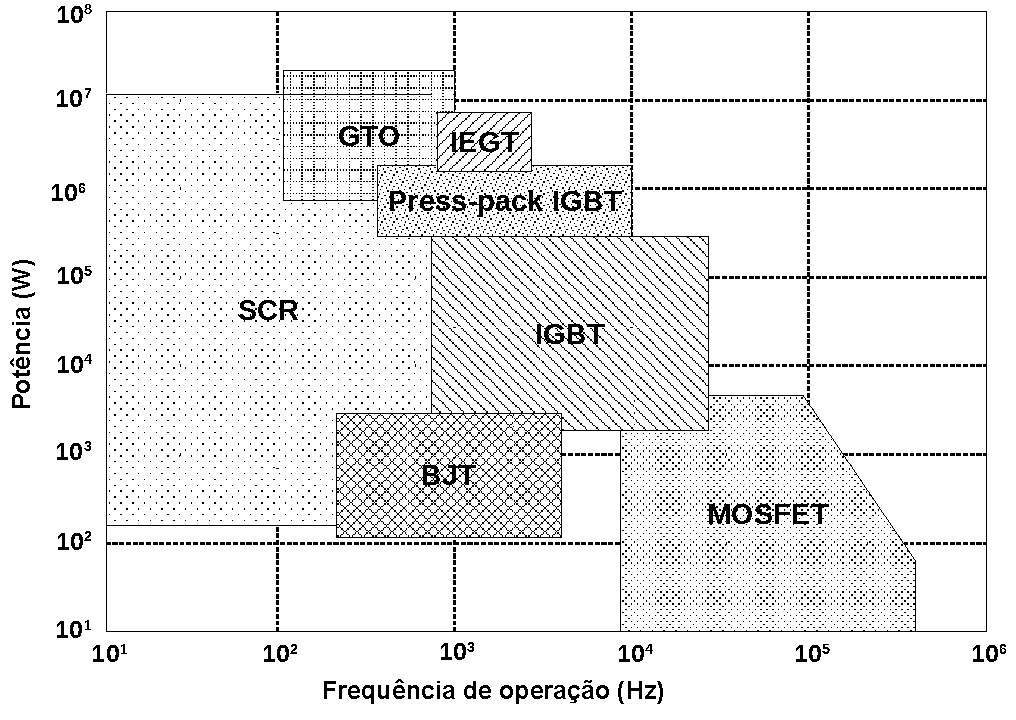
\includegraphics[scale=.9]{pdf/outros/diferenca_transistor2.pdf}
            	\label{fig:aplicacao_transistor}
             	\indentedfont[11cm]{Adaptado de \citeonline{ref:ELP_site_transistores}}
            \end{figure}
            
            \abreviatura'{MOSFET}{Metal Oxide Semiconductor Field Effect Transistor}{transistor de efeito de campo metal-óxido}
            
            Em conversores estáticos, com transistores operando como chave em alta frequência, para potências menores que \SI{1}{\kilo\watt}, comumente é utilizado transistores do tipo MOSFET (\textit{Metal Oxide Semiconductor Field Effect Transistor}, ou transistor de efeito de campo metal-óxido), uma vez que, como observado na \autoref{fig:aplicacao_transistor}, esses transistores operam em frequências mais elevadas \cite{ref:ELP_livro_ProjFontChav}. 
            % Por esse motivo, esse trabalho apenas abordará transistores MOSFET.
            
            Em um transistor MOSFET as perdas por condução, quando a chave está fechada, podem ser obtidas através da \autoref{eq:perda_cond_fet}. Essa equação utiliza para o cálculo a resistência intrínseca entre dreno e \textit{source} do transistor, comumente fornecida pelos fabricantes \cite{ref:ELP_livro_ProjFontChav}.
            
            \begin{equation} \label{eq:perda_cond_fet}
                \subx{P}{Tcond} = 
                \subx{R}{DS(on)}\cdot\subx{I}{Trms}^2
                %\frac{\subx{t}{on}}{\text{T}}\cdot\subx{R}{DS(on)}\cdot\subx{I}{d(on)}^2
            \end{equation}
            
            \begin{conditions}
                \subx{I}{Trms}      & Valor da corrente eficaz de dreno do transistor quando em condução (A) \\
                \subx{P}{Tcond}     & Perdas por condução no transistor (W) \\
                \subx{R}{DS(on)}    & Resistência equivalente entre dreno e \textit{source} do transistor (\ohm) 
            \end{conditions}
            
            Para as perdas por comutação do transistor MOSFET, semelhante ao diodo, deve-se levar em consideração que os tempos de acionamento e bloqueio para o caso não ideal são diferentes de zero. A \autoref{fig:perdas_mosfet_c} apresenta as principais medidas utilizadas para o cálculo das perdas por comutação, que levam em consideração os tempos de subida e descida, bem como a tensão entre dreno e \textit{Source} e a corrente no dreno do transistor \cite{ref:ELP_livro_ProjFontChav}. 
            
            \begin{figure}[H]
            	\centering
            	\caption{Comutação em um transistor MOSFET para uma carga resistiva}
            	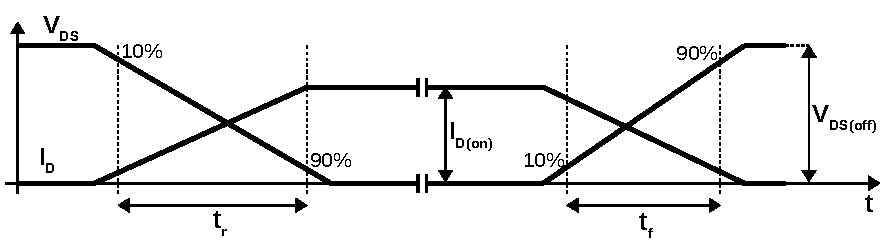
\includegraphics[scale=1]{pdf/perdas/perdas_transistor_c.pdf}
            	\label{fig:perdas_mosfet_c}
             	\indentedfont[15cm]{Adaptado de \citeonline[p.~166]{ref:ELP_livro_ProjFontChav}}
            \end{figure}
            
            O valor das perdas por comutação no MOSFET pode ser obtido através da \autoref{eq:perda_com_fet}. Sendo o valor das perdas totais igual soma das perdas por condução e das perdas por comutação \cite{ref:ELP_livro_ProjFontChav}.  
            
            \begin{equation} \label{eq:perda_com_fet}
                \subx{P}{Tcom} = 
                \frac{\text{f}}{2}\cdot(\subx{t}{r} + \subx{t}{f})\cdot\subx{I}{T(on)}\cdot\subx{V}{DS(off)}
            \end{equation}
            
            \begin{conditions}
                \text{f}            & Frequência de comutação do transistor (Hz) \\
                \subx{I}{T(on)}     & Corrente de dreno do transistor quando em condução (A) \\
                \subx{P}{Tcom}      & Perdas por comutação no transistor (W) \\
                \subx{t}{f}         & Tempo de descida da tensão de dreno-source do transistor (s) \\
                \subx{t}{r}         & Tempo de subida da tensão de dreno-source do transistor (s) \\
                \subx{V}{DS(off)}   & Tensão entre dreno e \textit{Source} do transistor (V)
            \end{conditions}
            
            \citeonline{ref:ELP_livro_ProjFontChav} afirma que para frequências muito baixas, como por exemplo \SI{60}{\hertz}, as perdas de comutação no diodo e no transistor podem ser ignoradas. Porém, na frequência de operação de conversores estáticos \mbox{CC-CC}, essas perdas tornam-se consideráveis, devido ao valor das perdas ser proporcional a frequência. Sendo assim, na escolha dos componentes, quanto menores forem os tempos de comutação dos semicondutores, menores serão as perdas. 
            
        %%%%%%%%%%%%%%%%%%%%%%%%%%%%%%%%%%%%%%%%%%%%%%%%%%%%%%%%%%%%%%%%%%%
        \subsection{Conversores \interleaved} \label{cap:fund_elp_inter}
        %%%%%%%%%%%%%%%%%%%%%%%%%%%%%%%%%%%%%%%%%%%%%%%%%%%%%%%%%%%%%%%%%%%
            
            Segundo \citeonline{ref:BI_phd_Peraca}, em projetos de conversores estáticos, há uma grande busca pelo aumento da eficiência energética e a redução do peso e volume. Assim, como mencionado na \autoref{cap:fund_elp_convlc_ccm}, uma alternativa para a redução dos elementos passivos de filtro consiste no aumento da frequência de chaveamento do conversor. Entretanto, tal aumento, como mostrado na \autoref{cap:fund_elp_convlc_perda}, ocasiona um acréscimo nas perdas por comutação.
            
            Com o crescimento da potência processada pelos conversores estáticos, cresce também a necessidade pela redução das perdas de condução. Pois, elevadas perdas de comutação e condução acarretam na redução do rendimento do conversor e um aumento do volume dos dissipadores \cite{ref:BI_phd_Peraca}.
            
            Para o processamento de potências elevadas, segundo \citeonline{ref:BI_phd_Peraca}, algumas técnicas podem ser utilizadas. Dentre elas, o uso de chaves ou conversores em série, ou ainda, conversores multiníveis em tensão, para os casos de conversores com tensões elevadas e o uso de chaves ou conversores em paralelo, ou conversores multiníveis em corrente, para os casos de conversores com correntes elevadas. Conciliando a aplicação com as tecnologias de semicondutores disponíveis, no que diz respeito a esforços de tensão e de corrente.
            
            Como uma alternativa para circuitos de alta corrente, surge a ideia dos conversores \interleaved. Esses conversores consistem em um método de colocar em paralelo N \abreviatura&{2SSC}{two-state switching cell}{células de comutação de dois estados} de conversores básicos, com mesma frequência de chaveamento e defasadas umas das outras \cite{ref:BI_artigo_DesignSimul}. 
            
            Para \citeonline{ref:BI_artigo_CarrBateria}, essa técnica, por dividir a corrente de saída do conversor em seus N ramos, reduz a amplitude da ondulação de corrente de saída e aumenta a sua frequência sem aumentar as perdas de comutação. Dessa forma, os conversores \interleaved apresentam requisitos de filtragem e armazenamento de energia menores se comparados aos conversores não \interleaved. Ainda, devido a divisão das correntes entre as chaves do conversor, há uma redução em seus esforços e uma melhor distribuição da potência processada. 
            
            Para um conversor do tipo Buck utilizando a técnica \interleaving com dois ramos, mostrado na \autoref{fig:c_buck_interl}, têm-se operando em paralelo os indutores, diodos e transistores. Nessa configuração o acionamento dos transistores $\subx{S}{1}$ e $\subx{S}{2}$ apresentam mesma frequência, porém defasados em \SI{180}{\degree} \cite{ref:BI_artigo_DesignSimul}.
            
            \begin{figure}[H]
            	\centering
            	\caption{Conversor Buck \interleaved de 2 ramos}
            	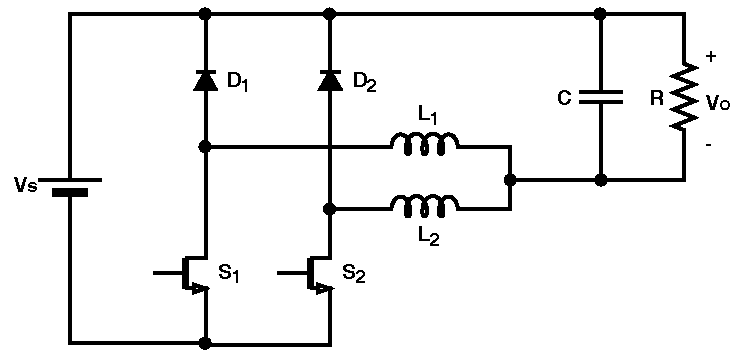
\includegraphics[scale=1]{pdf/interleaved/conversor_interleaved.pdf}
            	\label{fig:c_buck_interl}
             	\indentedfont[12.5cm]{Elaboração própria (2021)}
            \end{figure}
            
            Segundo \citeonline{ref:BI_artigo_CarrBateria}, devido à característica de divisão da corrente do \abreviatura.{CBI}{conversor \mbox{CC-CC} Buck \interleaved} em seus ramos, a sua corrente de saída apresentará uma ondulação de no máximo metade da ondulação de cada ramo, variando esse valor conforme a razão cíclica D. Assim, em um CBI a variação da corrente de saída será metade da corrente apresentada em um conversor Buck convencional (de apenas um ramo) com mesmas especificações de projeto.
            
            %%%%%%%%%%%%%%%%%%%%%%%%%%%%%%%%%%%%%%%%%%%%%%%%%%%%%%%%%%%%%%%%%%%
            \subsubsection{Projeto do filtro do conversor Buck \interleaved} \label{cap:fund_elp_inter_func}
            %%%%%%%%%%%%%%%%%%%%%%%%%%%%%%%%%%%%%%%%%%%%%%%%%%%%%%%%%%%%%%%%%%%
            
            \citeonline{ref:BI_artigo_DesignSimul} apresentam que a equação de projeto das indutâncias em um CBI de dois ramos operando em CCM é igual a utilizada no projeto de um conversor Buck convencional, como na \autoref{eq:buck_indutor}. 
            
            Porém, \citeonline{ref:BI_artigo_DesignSimul} advertem que, para o projeto do capacitor, deve-se considerar a frequência sobre o capacitor como o dobro da frequência de comutação e que a variação da corrente no indutor $\Delta\subx{I}{L}$ sobre o capacitor sofre uma atenuação. Dessa forma, a \autoref{eq:cbi_capacitor} apresenta a equação para o cálculo dessa capacitância. 
            
            \begin{equation} \label{eq:cbi_capacitor}
                \text{C} =
                \frac{ \frac{1-2\text{D}}{1-\text{D}}\cdot \Delta\subx{I}{L}}
                {16\cdot\text{f}\cdot\Delta\subx{V}{o}}
            \end{equation}
            
            \begin{conditions}
                \text{C}            & Capacitância (F) \\
                \text{D}            & Razão cíclica \\
                \text{f}            & Frequência de comutação do transistor (Hz) \\
                \Delta\subx{I}{L}   & Variação da corrente no indutor (A) \\
                \Delta\subx{V}{o}   & Variação da tensão de saída do conversor (V)
            \end{conditions}
            
            Para \citeonline{ref:BI_artigo_CarrBateria}, o valor da razão cíclica D, semelhante ao Buck convencional, pode ser obtido através da divisão da tensão de saída $\subx{V}{o}$ pela tensão de entrada $\subx{V}{s}$.
            
        %%%%%%%%%%%%%%%%%%%%%%%%%%%%%%%%%%%%%%%%%%%%%%%%%%%%%%%%%%%%%%%%%%%
        \subsection{Conversor Buck com célula de comutação de três estados} \label{cap:fund_elp_3ssc}
        %%%%%%%%%%%%%%%%%%%%%%%%%%%%%%%%%%%%%%%%%%%%%%%%%%%%%%%%%%%%%%%%%%%
            
            Para \citeonline{ref:BI_artigo_Falcondes}, uma variação dos circuitos com técnicas de \interleaving, consiste no uso de conversores com \abreviatura&{3SSC}{three-state switching cell}{célula de comutação de três estados}. A 3SSC, mostrado (a célula) na \autoref{fig:cell_3ssc}, pode ser obtida pela associação de duas 2SSC, como nos \interleaving, porém interconectada a um autotransformador com derivação central com relação de espiras unitárias. 
            
            \begin{figure}[H]
            	\centering
            	\caption{Célula de comutação de três estados}
            	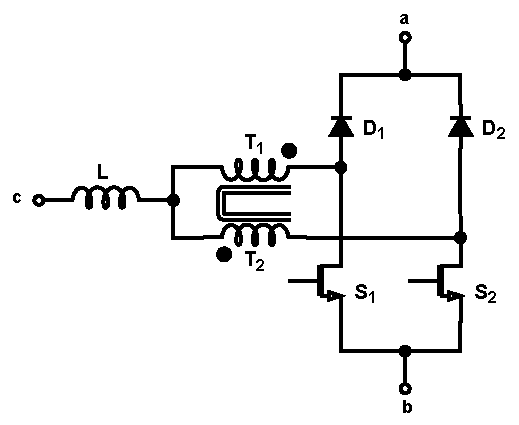
\includegraphics[scale=1]{pdf/interleaved/celula_3ssc_2.pdf}
            	\label{fig:cell_3ssc}
             	\indentedfont[9cm]{Elaboração própria (2021)}
            \end{figure}
            
            Conforme \citeonline{ref:BI_artigo_Falcondes}, o uso da 3SSC em conversores estáticos, devido ao autotransformador, acarreta em uma redução no dimensionamento do indutor L de armazenamento de energia e um maior equilíbrio nas correntes através de cada uma das chaves. A \autoref{fig:c_buck_3ssc} apresenta o conversor estático Buck utilizando a célula de comutação de três estados \cite{ref:BI_artigo_Falcondes}. 
            
            \begin{figure}[H]
            	\centering
            	\caption{Conversor Buck com célula de comutação de três estados}
            	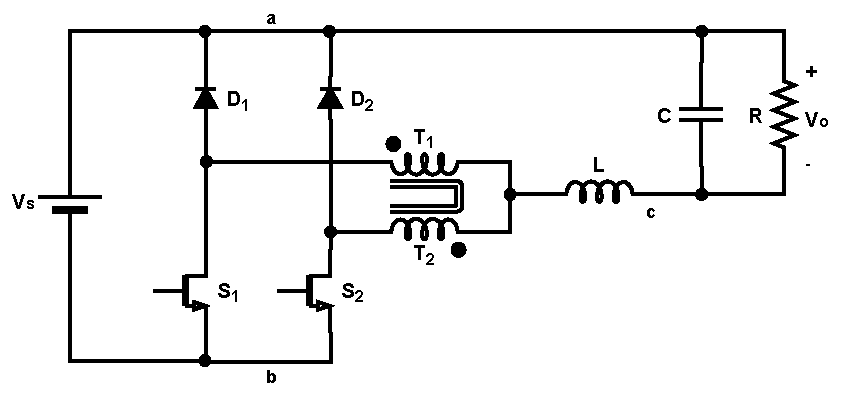
\includegraphics[scale=1]{pdf/interleaved/conversor_3SSC_2.pdf}
            	\label{fig:c_buck_3ssc}
             	\indentedfont[14cm]{Elaboração própria (2021)}
            \end{figure}
            
            Apesar da maior complexidade do circuito, com maior número de elementos se comparado ao Buck convencional, como as duas chaves $\subx{S}{1}$ e $\subx{S}{2}$, dois diodos $\subx{D}{1}$ e $\subx{D}{2}$, o autotransformador $\subx{T}{1}$ e $\subx{T}{2}$ e o indutor L, as vantagens obtidas com a estrutura são de grande interesse \cite{ref:BI_artigo_Falcondes}. 
            
            Essa abordagem proposta, segundo \citeonline{ref:BI_artigo_Balestero}, pode ser vista como a integração da técnica de \interleaving e da 3SSC. O autor ainda apresenta as seguintes características como vantagens da estrutura:
            
            \begin{alineas}
                \item tamanho, peso e volume reduzidos dos elementos magnéticos (indutores), projetados para o dobro da frequência de comutação, semelhante ao conversor Buck \interleaved;
                
                \item a corrente em cada braço é igual à metade da corrente total de saída, permitindo o uso de semicondutores com classificações de corrente mais baixas;
                
                \item melhor distribuição da dissipação térmica e, consequentemente, uso mais eficiente dos dissipadores de calor, devido às perdas serem distribuídas entre os semicondutores;
                
                \item metade da energia de entrada é diretamente transferida para a carga através dos diodos e dos indutores acoplados (autotransformadores), e não através das chaves. Podendo trazer melhoria, considerando diodos com melhores características elétricas relativas as perdas (condução e comutação) que os transistores;
                
                \item a potência é transferida da fonte para a carga durante a maior parte do período de comutação, diferentemente do que ocorre em conversores convencionais, ocorrendo apenas durante metade do período de comutação.
            \end{alineas}
            
            %%%%%%%%%%%%%%%%%%%%%%%%%%%%%%%%%%%%%%%%%%%%%%%%%%%%%%%%%%%%%%%%%%%
            \subsubsection{Projeto de um conversor Buck com 3SSC} \label{cap:fund_elp_3ssc_proj}
            %%%%%%%%%%%%%%%%%%%%%%%%%%%%%%%%%%%%%%%%%%%%%%%%%%%%%%%%%%%%%%%%%%%
            
            Para \citeonline{ref:BI_artigo_Falcondes}, o conversor buck utilizando 3SSC é capaz de operar em dois modos com relação as chaves. Se a razão cíclica D for maior que 0,5, o conversor opera no \abreviatura&{OM}{Overlapping mode}{modo sobreposto}, onde duas chaves permanecem ligadas simultaneamente. Caso contrário, se D<0,5, o conversor opera no \abreviatura&{NOM}{Nonoverlapping mode}{modo não sobreposto}, com apenas uma chave ligada por vez.
            
            \citeonline{ref:BI_artigo_Falcondes} afirma que, ao contrário do que ocorre no conversor Buck convencional, onde a análise dos estágios operacionais no CCM, DCM e CRM (\textit{Critical conduction mode}, ou modo de condução crítica) é válida para uma razão cíclica D com valores entre 0 e 1, o mesmo não acontece no conversor Buck baseado em 3SSC. Neste conversor, para \citeonline{ref:BI_artigo_Balestero} e \citeonline{ref:BI_artigo_Falcondes}, há uma necessidade de uma análise distinta para D<0,5 (NOM) e D>0,5 (OM). 
            
            \abreviatura'{CRM}{Critical conduction mode}{modo de condução crítica}
            
            Considerando o conversor operando em NOM, a \autoref{fig:c_buck_3ssc_estagio} apresenta as etapas de operação.
            
            \begin{figure}[H]
            	\centering
            	\caption{Estágios de operação de um conversor Buck baseado em 3SSC}
            	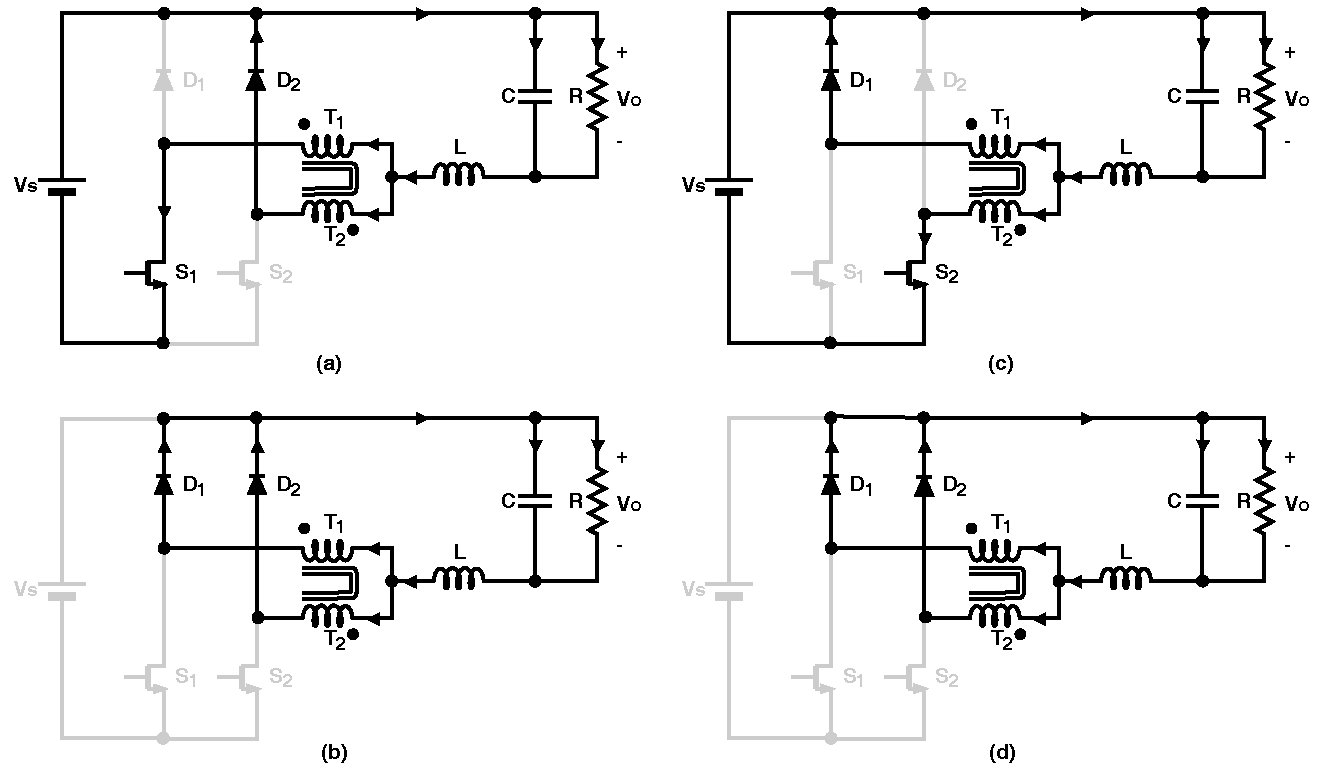
\includegraphics[scale=.7]{pdf/interleaved/estag_oper_3ssc.pdf}
            	\label{fig:c_buck_3ssc_estagio}
             	\indentedfont[16cm]{Adaptado de \citeonline{ref:BI_artigo_Balestero}}
            \end{figure}
            
            Como já mencionado, neste modo de operação, as chaves $\subx{S}{1}$ e $\subx{S}{2}$ não acionam simultaneamente. Assim, tem-se que: 
            
            \begin{alineas}
                \item na primeira etapa, a chave $\subx{S}{1}$ e o diodo $\subx{D}{2}$ estão conduzindo e a fonte $\subx{V}{S}$ fornecendo a energia para a carga, conforme \autoref{fig:c_buck_3ssc_estagio}a;
                
                \item na segunda etapa, \autoref{fig:c_buck_3ssc_estagio}b, ambas as chaves estão em aberto e apenas os diodos conduzem e o indutor é responsável por fornecer a energia;
                
                \item na terceira etapa, a chave $\subx{S}{2}$ e o diodo $\subx{D}{1}$ passam a conduzir e a fonte $\subx{V}{S}$ volta a fornecer a energia para a carga, como na \autoref{fig:c_buck_3ssc_estagio}c;
                
                \item na quarta etapa, semelhante ao estágio da \autoref{fig:c_buck_3ssc_estagio}b, na \autoref{fig:c_buck_3ssc_estagio}d, apenas os diodos estão conduzindo e o indutor fornece a energia para a carga.
            \end{alineas}
            
            
            Nesse conversor, \citeonline{ref:BI_tcc_Balestero} demonstra que ao operar na região do CCM, sua indutância será um quarto da indutância necessária em um conversor Buck convencional com mesma especificação de projeto. O valor da indutância para o projeto de filtro do conversor pode ser obtido através da \autoref{eq:3ssc_indutor}.  
            
            \begin{equation} \label{eq:3ssc_indutor}
                \text{L} = 
                \frac{(\subx{V}{s} - 2\cdot\subx{V}{o})\cdot\text{D}}
                {2\cdot\text{f}\cdot\Delta\subx{I}{L}}
            \end{equation}
            
            \begin{conditions}
                \text{D}            & Razão cíclica \\
                \text{f}            & Frequência de comutação do transistor (Hz) \\
                \Delta\subx{I}{L}   & Variação da corrente no indutor (A) \\
                \text{L}            & Indutância (H) \\
                \subx{V}{o}         & Tensão de saída do conversor (V) \\
                \subx{V}{s}         & Tensão de entrada do conversor (V) 
            \end{conditions}
            
            \citeonline{ref:BI_tcc_Balestero} apresenta para o projeto do valor da capacitância de filtro do conversor a \autoref{eq:3ssc_capacitor}, similar as equações anteriores de capacitância. 
            
            \begin{equation} \label{eq:3ssc_capacitor}
                \text{C} =
                \frac{\Delta\subx{I}{L}}
                {4\cdot\pi\cdot\text{f}\cdot\Delta\subx{V}{o}}
            \end{equation}
            
            \begin{conditions}
                \text{C}            & Capacitância (F) \\
                \text{f}            & Frequência de comutação do transistor (Hz) \\
                \Delta\subx{I}{L}   & Variação da corrente no indutor (A) \\
                \Delta\subx{V}{o}   & Variação da tensão de saída do conversor (V)
            \end{conditions}
            
    %%%%%%%%%%%%%%%%%%%%%%%%%%%%%%%%%%%%%%%%%%%%%%%%%%%%%%%%%%%%%%%%%%%
    \section{Compatibilidade eletromagnética} \label{cap:fund_emc}
    %%%%%%%%%%%%%%%%%%%%%%%%%%%%%%%%%%%%%%%%%%%%%%%%%%%%%%%%%%%%%%%%%%%
    
    Para atuar na resolução de problemas de compatibilidade eletromagnética em conversores estáticos, se faz necessário conceituar a EMC e a \abreviatura&{EMI}{Electromagnetic interference}{interferência eletromagnética}.
    
    \citeonline{ref:EMC_livro_Paul} afirma que um sistema ou grupo de sistemas eletrônicos que sejam capazes de funcionar de forma compatível entre si e não produzir ou ser suscetível a interferências é considerado eletromagneticamente compatível com seu ambiente. Assim, o autor afirma que um sistema é eletromagneticamente compatível quando satisfaz os três seguintes critérios:
    
    \begin{citacao}
        \begin{enumerate}[leftmargin=\leftskip+\labelwidth-\labelsep]
            \item não causar interferência em outros sistemas;
            \item não ser suscetível a emissões de outros sistemas;
            \item não causar interferência em si mesmo. \cite[p.~2, tradução nossa]{ref:EMC_livro_Paul}.
        \end{enumerate}
    \end{citacao}
    
    Para \citeonline{ref:EMC_livro_Paul}, a estrutura básica de qualquer problema de EMC, como mostrado na \autoref{fig:gerar_meio_recept}, é composta por um sistema gerador da interferência, um sistema suscetível a interferência (receptor) e um meio de propagação da interferência (da fonte até o receptor).
    
    \begin{figure}[H]
    	\centering
    	\caption{Estrutura básica do problema de acoplamento eletromagnético}
    	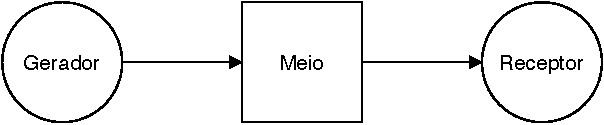
\includegraphics[scale=1]{pdf/outros/gera_meio_recep.pdf}
    	\label{fig:gerar_meio_recept}
     	\indentedfont[10.5cm]{Adaptado de \citeonline[p.~3]{ref:EMC_livro_Paul}}
    \end{figure}
    
    Dessa forma, \citeonline{ref:EMC_livro_PrintedCircuit} afirma que a falta de compatibilidade eletromagnética em um sistema, em essência, é a interferência eletromagnética. A EMI é o processo pelo qual a energia eletromagnética, associada ao ruído gerado pelo sistema, é transmitida de um dispositivo eletrônico para outro, seja de forma irradiada através do ar ou conduzida por meios condutores (ou ambos). 
    
    Assim, para que se tenha um bom funcionamento de sistemas em um determinado ambiente, é necessário que os sistemas presentes sejam eletromagneticamente compatíveis. No qual necessita-se reduzir os níveis de EMI gerados e absorvidos até valores aceitáveis. Para tal, \citeonline{ref:EMC_livro_Paul} afirma que deve-se adotar os seguintes procedimentos: 
    
    \begin{citacao}
        \begin{enumerate}[leftmargin=\leftskip+\labelwidth-\labelsep]
            \item suprimir a emissão gerada;
            \item tornar o meio de acoplamento o mais ineficiente possível;
            \item tornar o receptor menos suscetível à emissão. \cite[p.~4, tradução nossa]{ref:EMC_livro_Paul}.
        \end{enumerate}
    \end{citacao}
    
    Ainda, \citeonline{ref:EMC_livro_Paul} salienta que um determinado sistema que gera uma frequência ou faixa de frequências, tende a ser suscetível a esta frequência ou faixa de frequências.
    
    Para \citeonline{ref:EMC_phd_schlichting}, a propagação da energia eletromagnética entre sistemas pode ser classificada em: emissão conduzida, suscetibilidade a condução, emissão irradiada e suscetibilidade a irradiação.
    
        %%%%%%%%%%%%%%%%%%%%%%%%%%%%%%%%%%%%%%%%%%%%%%%%%%%%%%%%%%%%%%%%%%%
        \subsection{Gerador} \label{cap:fund_emc_gen}
        %%%%%%%%%%%%%%%%%%%%%%%%%%%%%%%%%%%%%%%%%%%%%%%%%%%%%%%%%%%%%%%%%%%
        
        Em projetos de circuitos eletrônicos, como já mencionado, há uma crescente busca por elementos semicondutores com características de tempos de subida e descida menores. Porém, o aumento da frequência de comutação com semicondutores mais rápidos, segundo \citeonline{ref:EMC_phd_schlichting}, ocasiona em problemas para a EMC dos produtos, por estes gerarem uma comutação com conteúdo harmônico mais amplo.
        
        Este comportamento não linear da comutação de tensões e correntes em frequências elevadas, produzem distúrbios de alta frequência que podem se propagar pelo equipamento, carga, rede de alimentação e pelo ar. Dessa forma, em produtos eletrônicos, os maiores geradores de ruídos são os componentes responsáveis pela comutação, como diodos e transistores, tornando os conversores estáticos grandes fontes geradoras de EMI \cite{ref:EMC_phd_schlichting}. 
        
        O espectro harmônico é a representação de um sinal temporal no domínio da frequência. Assim, o espectro harmônico de um sinal comutado pode ser observado na \autoref{fig:sinal_comut_ideal_real}. A \autoref{fig:sinal_comut_ideal} apresenta um sinal comutado ideal, com um pulso com tempo de subida e descida nulo. Na \autoref{fig:sinal_comut_real} é apresentado um sinal comutado real, com tempos de subida e descida diferentes de zero. Na figura, os tempos de subida e descida são considerados iguais, o que geralmente não acontece em um sinal prático \cite{ref:EMC_phd_schlichting}.
        
        \begin{figure}[H]
            \centering
            \caption{Espectro harmônico de um pulso}
            \begin{subfigure}[H]{.49\textwidth}
                \centering
                \caption{tempo de subida e de decida nulos}
                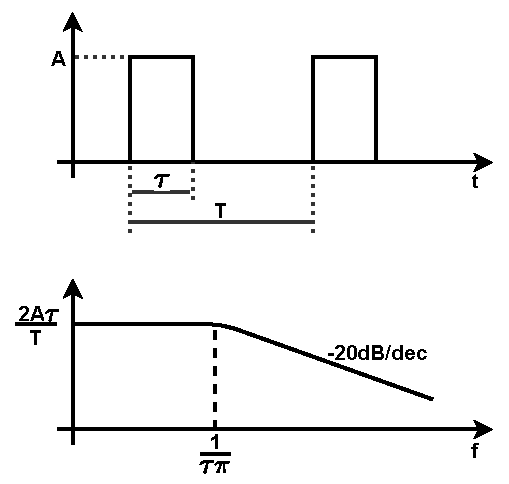
\includegraphics[scale=.9]{pdf/outros/sinal_comut_ideal.pdf}
                \label{fig:sinal_comut_ideal}
            \end{subfigure}
            \begin{subfigure}[H]{.49\textwidth}
                \centering
                \caption{tempo de subida e decida não nulos}
                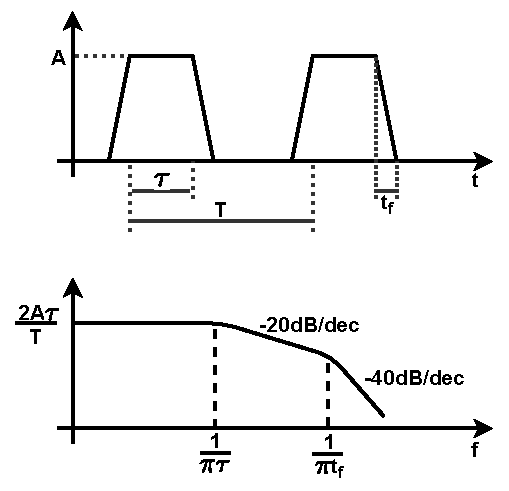
\includegraphics[scale=.9]{pdf/outros/sinal_comut_real.pdf}
                \label{fig:sinal_comut_real}
            \end{subfigure}
            \indentedfont[15.5cm]{Adaptado de \citeonline[p.~34]{ref:EMC_phd_schlichting}}
        	\label{fig:sinal_comut_ideal_real}
        \end{figure}
        
        \begin{conditions}
            \text{A}            & Amplitude do sinal \\
            %\text{D}            & Tempo de condução \\
            \tau                & Período de condução (s) \\
            \text{T}            & Período total (s) \\
            \subx{t}{f}         & Tempo de comutação (s) 
        \end{conditions}
        
        Percebe-se pela figura a influência do período de condução no espectro harmônico do sinal e, para um sinal com tempos de comutação diferentes de zero, a influência do tempo de comutação na atenuação do espectro harmônico após a frequência $\frac{1}{\pi\subx{t}{f}}$. Ainda, quanto maior é a amplitude do sinal comutado maior é a amplitude do espectro harmônico gerado na comutação.
        
        %%%%%%%%%%%%%%%%%%%%%%%%%%%%%%%%%%%%%%%%%%%%%%%%%%%%%%%%%%%%%%%%%%%
        \subsubsection{Diodos como elementos geradores de EMI} \label{cap:fund_emc_gen_diodo}
        %%%%%%%%%%%%%%%%%%%%%%%%%%%%%%%%%%%%%%%%%%%%%%%%%%%%%%%%%%%%%%%%%%%
        
        A geração de ruído em um diodo, segundo \citeonline{ref:EMC_phd_schlichting}, se dá devido aos seus transitórios de tensão e corrente. A \autoref{fig:EMC_diodo_EBcond} apresenta o comportamento dinâmico típico da tensão e corrente no diodo operando como comutador. 
        
        \begin{figure}[H]
            \centering
            \caption{Comportamento dinâmico típico da tensão e corrente de um diodo}
            \begin{subfigure}[H]{.49\textwidth}
                \centering
                \caption{Tempo de entrada em condução}
                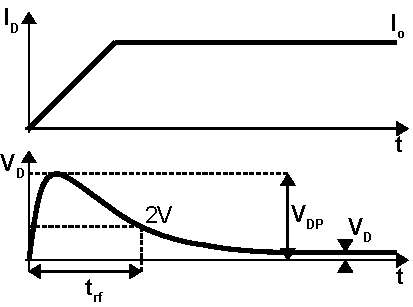
\includegraphics[scale=1]{pdf/perdas/perdas_diodo_c1_p.pdf}
                \label{fig:EMC_diodo_Econd}
            \end{subfigure}
            \begin{subfigure}[H]{.49\textwidth}
                \centering
                \caption{Tempo de bloqueio}
                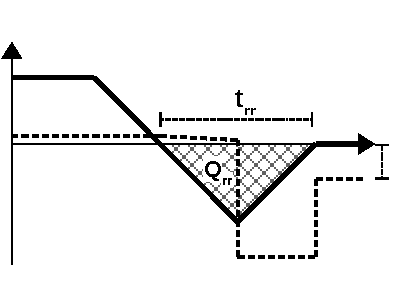
\includegraphics[scale=1]{pdf/perdas/perdas_diodo_c2_p.pdf}
                \label{fig:EMC_diodo_Bcond}
            \end{subfigure}
            \indentedfont[15.5cm]{Adaptado de \citeonline[p.~6~e~8]{ref:ELP_livro_EletrPotBarbi}}
        	\label{fig:EMC_diodo_EBcond}
        \end{figure}
        
        \begin{conditions}
            \subx{I}{o}         & Corrente do diodo em condução (A) \\
            \subx{Q}{rr}        & Carga do capacitor intrínseco do diodo (\si{\coulomb}) \\
            \subx{t}{rf}        & Tempo de atraso na transição (s) \\
            \subx{t}{rr}        & Tempo de recuperação reversa do diodo (s) \\
            \subx{V}{D}         & Tensão do diodo em condução (V) \\
            \subx{V}{DP}        & Tensão de pico do diodo na entrada em condução (V)
        \end{conditions}
        
        Como observado, na entrada em condução do diodo (\autoref{fig:EMC_diodo_Econd}), tem-se um crescimento rápido da corrente $\subx{I}{D}$. Porém, por não ser instantâneo, nesse pequeno intervalo de tempo $\subx{t}{rf}$, ocorre um pico de tensão $\subx{V}{DP}$ no diodo. Esse tempo ocorre devido à características de cada diodo, com os tempos e amplitudes variando de diodo para diodo. Apesar desse pico de tensão possuir uma larga faixa de emissão, o mesmo não possui uma grande energia associada \cite{ref:EMC_phd_schlichting}. 
        
        Porém, na parte do bloqueio (\autoref{fig:EMC_diodo_Bcond}), a EMI produzida é maior. Como mencionado na \autoref{cap:fund_elp_convlc_perda}, no bloqueio, devido às capacitâncias intrínsecas do diodo e características indutivas do circuito, ocorrem picos de tensão e corrente reversa sobre o mesmo, com elevadas amplitudes e derivadas de corrente. Devido a essas elevadas amplitudes e derivadas de corrente, a energia associada ao bloqueio geralmente é bem maior do que na entrada em condução \cite{ref:EMC_phd_schlichting}.
        
        %%%%%%%%%%%%%%%%%%%%%%%%%%%%%%%%%%%%%%%%%%%%%%%%%%%%%%%%%%%%%%%%%%%
        \subsubsection{Transistores como elementos geradores de EMI} \label{cap:fund_emc_gen_trans}
        %%%%%%%%%%%%%%%%%%%%%%%%%%%%%%%%%%%%%%%%%%%%%%%%%%%%%%%%%%%%%%%%%%%
        
        Semelhante aos diodos, os transistores, por serem empregados como comutadores, são grandes fontes geradoras de ruído. Dado o modo de operação dos transistores, através do controle da entrada em condução e bloqueio, segundo \citeonline{ref:EMC_phd_schlichting}, os mesmos podem apresentar níveis elevados de emissão tanto no bloqueio quanto na entrada em condução, diferente dos diodos.
        
        Para \citeonline{ref:EMC_phd_schlichting}, os transistores apresentam um espectro harmônico geralmente maior que o gerado pelos diodos, devido à essa energia associada ao bloqueio e entrada em condução ser maior. Isto ocorre por que quase sempre se tem uma alta derivada de tensão nas comutações.
        
        A EMI gerada, proveniente dos tempos, formas de onda e amplitudes das tensões e correntes, dependem das características construtivas dos transistores (como capacitâncias intrínsecas) e das características do circuito (como impedâncias, níveis de tensão e corrente da comutação, entre outros) \cite{ref:EMC_phd_schlichting}.
        
        %%%%%%%%%%%%%%%%%%%%%%%%%%%%%%%%%%%%%%%%%%%%%%%%%%%%%%%%%%%%%%%%%%%
        \subsection{Receptor} \label{cap:fund_emc_recep}
        %%%%%%%%%%%%%%%%%%%%%%%%%%%%%%%%%%%%%%%%%%%%%%%%%%%%%%%%%%%%%%%%%%%
        
        Como já mencionado, um circuito eletrônico pode ser classificado como gerador de EMI e/ou como receptor. Dessa forma, \citeonline{ref:EMC_livro_Paul} afirma que um equipamento que produz interferência eletromagnética, também é suscetível a mesma faixa de frequência, seja ela oriunda de fontes externas ou dele próprio. 
        
        Para \citeonline{ref:EMC_phd_schlichting}, na EMI conduzida a propagação e recepção se dá pela conexão do circuito com a rede e a carga, através dos cabos de alimentação e do plano de terra, seja nos modos comum ou diferencial. Para a emissão e recepção de EMI irradiadas, têm-se fios, trilhas e caminhos fechados (\textit{loop}) atuando como antenas.
        
        %%%%%%%%%%%%%%%%%%%%%%%%%%%%%%%%%%%%%%%%%%%%%%%%%%%%%%%%%%%%%%%%%%%
        \subsection{Interferência conduzida} \label{cap:fund_emc_intcond}
        %%%%%%%%%%%%%%%%%%%%%%%%%%%%%%%%%%%%%%%%%%%%%%%%%%%%%%%%%%%%%%%%%%%
        
        A condução, segundo \citeonline{ref:EMC_msc_muriel}, é a forma pelo qual o ruído eletromagnético produzido é levado para dentro ou para fora de um sistema via condutores metálicos ou elementos parasitas. Esses caminhos de propagação da EMI conduzida podem ser intencionais, como através de trilhas e componentes, e/ou não intencionais, como capacitâncias intrínsecas de componentes e acoplamentos capacitivos e indutivos. Por esse motivo, a redução da emissão conduzida torna-se uma tarefa trabalhosa e complexa, uma vez que necessita do conhecimento de todos os possíveis caminhos percorridos pelo ruído para se propagar para dentro e/ou para fora de um equipamento \cite{ref:EMC_phd_schlichting}. 
        
        Essa interferência ainda pode ser dividida em duas componentes, podendo ser propagada através de correntes de modo comum e/ou correntes de modo diferencial.
        %Essa interferência ainda pode se propagar através de correntes de modo comum e/ou correntes de modo diferencial. 
        Como apresentado na \autoref{fig:corrente_comum_dif}, as correntes de modo comum ($\subx{I}{mc}$) são aquelas que se propagam no mesmo sentido de propagação em cabos e trilhas e as correntes de modo diferencial ($\subx{I}{md}$) são aquelas que se propagam em sentidos opostos. 
        
        % Schlichting - p. 40
        \begin{figure}[H]
        	\centering
        	\caption{Correntes de modo comum e diferencial}
        	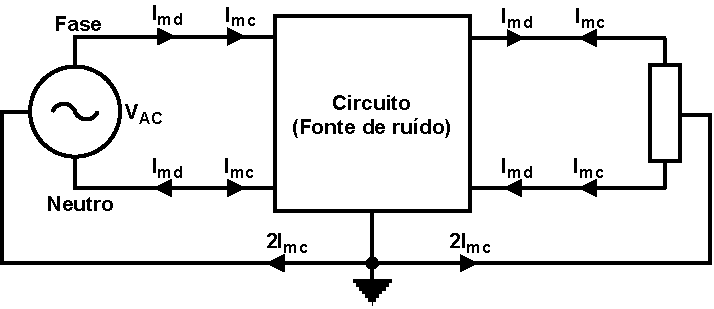
\includegraphics[scale=1]{pdf/outros/gerador_ruido.pdf}
        	\label{fig:corrente_comum_dif}
         	\indentedfont[12cm]{Adaptado de \citeonline[p.~40]{ref:EMC_phd_schlichting}}
        \end{figure}
        
        Como observado na \autoref{fig:corrente_comum_dif}, as correntes de modo diferencial ($\subx{I}{md}$) circulam entre os condutores de fase e neutro que conectam o circuito à rede de alimentação e entre os condutores que conectam o mesmo à carga. Já as correntes de modo comum ($\subx{I}{mc}$) circulam entre os condutores de fase e neutro e o plano de referência (terra) e entre os condutores que conectam o circuito à carga e o plano de referência. Sendo que essa conexão com o plano de referência ocorre mesmo que não haja conexão metálica com o mesmo \cite{ref:EMC_phd_schlichting}. 
        
        %%%%%%%%%%%%%%%%%%%%%%%%%%%%%%%%%%%%%%%%%%%%%%%%%%%%%%%%%%%%%%%%%%%
        \subsection{Interferência irradiada} \label{cap:fund_emc_intirrad}
        %%%%%%%%%%%%%%%%%%%%%%%%%%%%%%%%%%%%%%%%%%%%%%%%%%%%%%%%%%%%%%%%%%%
        
        A radiação é a forma pelo qual o ruído eletromagnético produzido é levado para dentro ou fora de um sistema via meios não metálicos, como o ar. O ruído irradiado é gerado, em sua maioria, devido à circulação de correntes por trilhas, cabos, terminais de semicondutores e caminhos fechados (\textit{loop}), que geram campos eletromagnéticos com parâmetros dependentes da amplitude e frequência dessa corrente, dimensões das trilhas e/ou cabos, área do \textit{loop}, entre outros \cite{ref:EMC_msc_muriel}.
        
        Como na interferência conduzida, na irradiada, o trabalho para mitigação desse ruído é uma tarefa trabalhosa e complexa, por exigir o conhecimento do comportamento eletromagnético em alta frequência dos materiais presentes no sistema \cite{ref:EMC_phd_schlichting}.
        
        %%%%%%%%%%%%%%%%%%%%%%%%%%%%%%%%%%%%%%%%%%%%%%%%%%%%%%%%%%%%%%%%%%%
        \subsection{Normas de compatibilidade eletromagnética} \label{cap:fund_emc_norma}
        %%%%%%%%%%%%%%%%%%%%%%%%%%%%%%%%%%%%%%%%%%%%%%%%%%%%%%%%%%%%%%%%%%%
        
        Devido ao aumento do número de equipamentos eletrônicos, e consequentemente, o aumento dos problemas de EMC entre eles, fez-se necessário a criação de normas para regulamentar esses equipamentos. Sendo as medidas de emissão irradiada e conduzida complexas, essas normas visam padronizar os procedimentos de testes e unidades de medida para que seja possível a comparação dos resultados obtidos em locais e processos diferentes. Essas normas de EMC podem ser divididas em normas impostas pelas agências governamentais e normas impostas pelos próprios fabricantes dos equipamentos \cite{ref:EMC_phd_schlichting}. 
        
        As normas de EMC impostas pelas agências governamentais são normas legais e obrigatórias, criadas para controlar tanto a interferência produzida por determinado equipamento quanto a suscetibilidade dele. Já as normas de EMC impostas pelos fabricantes são normas que os mesmos impões visando um equipamento mais confiável e de qualidade.
        
        Dessa forma, com o intuito de uma maior padronização, e apesar de não ser uma agência normatizadora, o \abreviatura&{CISPR}{Comité International Spécial des Perturbations Radioélectriques}{Comitê Internacional Especial de Rádio Interferência} têm frequentemente suas normas sendo adotadas por países e órgãos reguladores \cite{ref:EMC_iec_about, ref:EMC_phd_schlichting}.
        
            %%%%%%%%%%%%%%%%%%%%%%%%%%%%%%%%%%%%%%%%%%%%%%%%%%%%%%%%%%%%%%%%%%%
            \subsubsection{Formas de medição} \label{cap:fund_emc_norma_medicao}
            %%%%%%%%%%%%%%%%%%%%%%%%%%%%%%%%%%%%%%%%%%%%%%%%%%%%%%%%%%%%%%%%%%%
            % Equipamentos usados
             
            De modo geral, as normas para emissão irradiada estabelecem que as medidas feitas no equipamento devem ser realizadas, preferencialmente, em campo aberto. Porém, devido a dificuldade de se encontrar um local livre de radiação para realizar as medidas, tem-se como alternativa o uso de câmaras anecoicas ou semi-anecoicas. Essas câmaras têm como característica um ambiente blindado eletromagneticamente para evitar que sinais externos contaminem o teste e possuem paredes e teto cobertos por cones de absorção de radiofrequência que simulam um local em espaço aberto e evitando reflexões nas paredes e teto das emissões \cite{ref:EMC_phd_schlichting, ref:EMC_livro_Paul}. 
            
            Segundo \citeonline{ref:EMC_livro_Paul}, dentro da câmara, uma antena de ampla banda é posicionada para realizar a medição da radiação do equipamento. Sendo essa antena conectada a um analisador de espectro que registra o nível de ruído emitido em cada frequência. A \autoref{fig:camara_semi_anecoica} ilustra os elementos presentes em uma câmara semi-anecoica. 
            
            \begin{figure}[H]
            	\centering
            	\caption{Representação de uma câmara semi-anecoicas para a medição das emissões irradiadas}
            	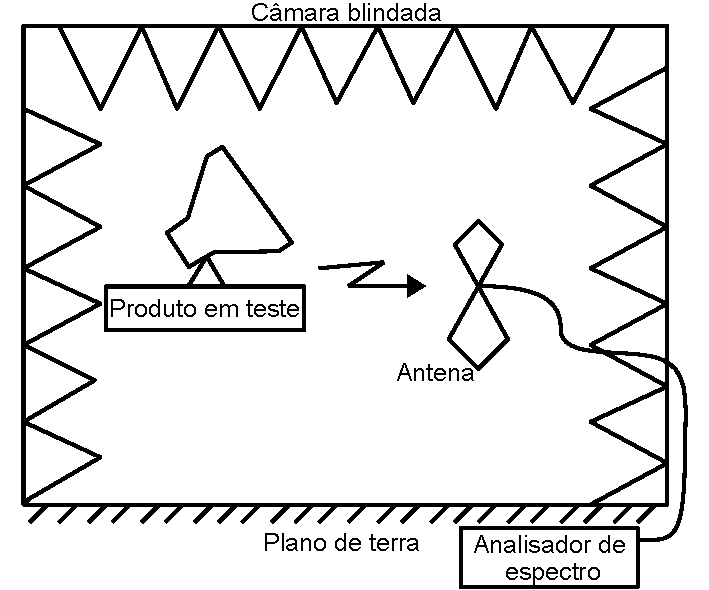
\includegraphics[scale=1]{pdf/outros/camaca_emc.pdf}
            	\label{fig:camara_semi_anecoica}
             	\indentedfont[12cm]{Adaptado de \citeonline[p.~66]{ref:EMC_livro_Paul}}
            \end{figure}
            
            Para a emissão conduzida, segundo \citeonline{ref:EMC_phd_schlichting}, o equipamento a ser testado deve estar isolado da rede de alimentação. Para tal, é utilizado entre o equipamento sob teste e a rede de alimentação uma \abreviatura&{LISN}{Line Impedance Stabilization Network}{rede de estabilização de impedância de linha}. A LISN tem como finalidade evitar que ruídos externos provenientes da rede de energia contaminem a medida, apresentar uma impedância constante de \SI{50}{$\Omega$} entre os fios de fase e terra e entre os fios neutro e terra e atuar como transdutor de corrente interferente para tensão interferente. A \autoref{fig:meidcao_lisn} apresenta a configuração típica de teste utilizando a LISN. 
            
            % Schlichting - p. 40
            \begin{figure}[H]
            	\centering
            	\caption{Representação de uma LISN na medição das emissões conduzidas}
            	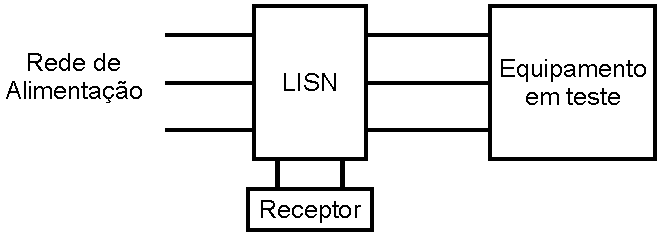
\includegraphics[scale=1]{pdf/outros/lisn_modelo.pdf}
            	\label{fig:meidcao_lisn}
             	\indentedfont[12cm]{Adaptado de \citeonline[p.~16]{ref:EMC_phd_schlichting}}
            \end{figure}
            
            Dessa forma, qualquer corrente que circule pelo cabo de alimentação do equipamento é medida pela LISN, desde que esteja dentro da faixa de frequência a ser medida. Vale observar que todas as medidas das emissões irradiadas e conduzidas devem ser realizadas com o sistema completo, isto é, com todos os cabos de conexão e subsistemas conectados \cite{ref:EMC_phd_schlichting}.
            
            
            %%%%%%%%%%%%%%%%%%%%%%%%%%%%%%%%%%%%%%%%%%%%%%%%%%%%%%%%%%%%%%%%%%%
            \subsubsection{Norma de EMC aplicáveis ao projeto} \label{cap:fund_emc_norma_proj}
            %%%%%%%%%%%%%%%%%%%%%%%%%%%%%%%%%%%%%%%%%%%%%%%%%%%%%%%%%%%%%%%%%%%
            
            Como mencionado, as normas internacionais desenvolvidas pelo CISPR tem sido adotada como um padrão único para as normas internacionais de EMC. Dentre as normas criadas, tem-se a publicação Número 22 (CISPR22), que engloba os equipamentos de tecnologia da informação, incluindo dispositivos digitais \cite{ref:EMC_phd_schlichting}. 
            Por esta razão, devido ao projeto desenvolvido não possuir aplicação definida, e sendo conversores estáticos comumente enquadrados nesta norma, a mesma foi utilizada de forma a facilitar a visualização dos resultados obtidos. 
            
            O CISPR divide os equipamentos em duas classes: classe A e classe B. Sendo os equipamentos classe A de uso industrial e os de classe B de uso residencial. A \autoref{fig:cispr22_irrad} apresenta os limites impostos pela CISPR22 de emissão irradiada para equipamentos classe B. Como pode ser observado, a  faixa de frequência avaliada pela norma para emissões irradiada é de \SI{30}{\mega\hertz} a  \SI{1}{\giga\hertz}.
            
            \begin{figure}[H]
            	\centering
            	\caption{Limites de emissões irradiada impostas pela CISPR22 para equipamentos classe B}
            	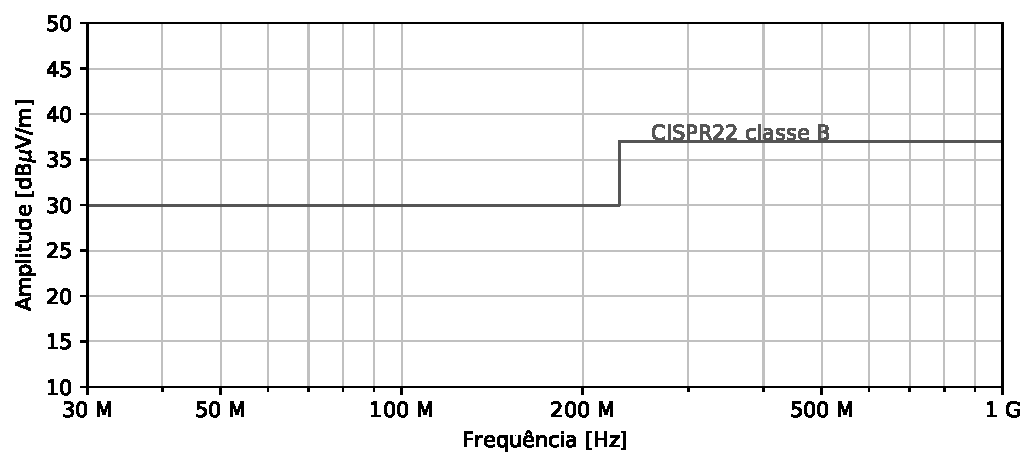
\includegraphics[scale=.9]{pdf/rad/norma_rad.pdf}
            	\label{fig:cispr22_irrad}
             	\indentedfont[15.5cm]{Adaptado de \citeonline{ref:EMC_CISPR22}}
            \end{figure}
            
            Para a emissão conduzida, a faixa de frequência avaliada pela CISPR22 é de \SI{150}{\kilo\hertz} a  \SI{30}{\mega\hertz}. A \autoref{fig:cispr22_cond} apresenta os limites impostos pela CISPR22 de emissão conduzida para equipamentos classe B, para medidas quando o receptor de EMC utiliza um detector de Quase-Pico (QP).
            
            \begin{figure}[H]
            	\centering
            	\caption{Limites de emissões conduzidas impostas pela CISPR22 para equipamentos classe B}
            	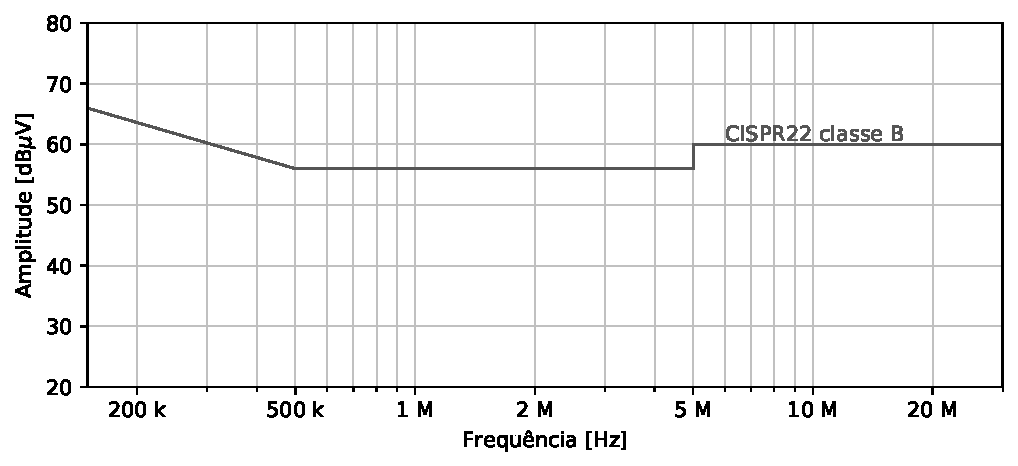
\includegraphics[scale=.9]{pdf/cond/norma_cond.pdf}
            	\label{fig:cispr22_cond}
             	\indentedfont[15.5cm]{Adaptado de \citeonline{ref:EMC_CISPR22}}
            \end{figure}
            
            %%%%%%%%%%%%%%%%%%%%%%%%%%%%%%%%%%%%%%%%%%%%%%%%%%%%%%%%%%%%%%%%%%%
            \subsection{Técnicas para mitigação de ruído} \label{cap:fund_emc_conv_mitig}
            %%%%%%%%%%%%%%%%%%%%%%%%%%%%%%%%%%%%%%%%%%%%%%%%%%%%%%%%%%%%%%%%%%%
            
            Como mencionado na subseção anterior, a redução dos níveis de EMI é de grande importância tanto para o correto funcionamento do equipamento quanto para que o fabricante do equipamento tenha aprovação para revenda do mesmo. Devendo não só buscar esta redução para satisfazer as normas legais, mas também para atender as expectativas dos usuários. %\citeonline{ref:EMC_phd_schlichting}
            
            Em sua maioria, exceto nos casos mais simples, uma solução única para um determinado problema de EMC pode não existir, geralmente sendo necessárias uma composições de técnicas \cite{ref:EMC_livro_NoiseReduct}. Segundo \citeonline{ref:EMC_phd_schlichting}, essas técnicas buscam minimizar a EMI, uma vez que não é possível eliminar tal interferência.
            
            Ainda, \citeonline{ref:EMC_phd_schlichting} afirma que alguns desses problemas de interferência podem ser resolvidos ainda em etapas anteriores do projeto, ganhando tempo e reduzindo os investimentos necessários. 
            
            %%%%%%%%%%%%%%%%%%%%%%%%%%%%%%%%%%%%%%%%%%%%%%%%%%%%%%%%%%%%%%%%%%%
            \subsubsection{Layout de placa de circuito impresso} \label{cap:fund_emc_conv_mitig_cond}
            %%%%%%%%%%%%%%%%%%%%%%%%%%%%%%%%%%%%%%%%%%%%%%%%%%%%%%%%%%%%%%%%%%
            
            Segundo as equações de Maxwell, uma corrente que seja alternada no tempo produz um campo eletromagnético. Isso ocorre em todo condutor elétrico, que por não serem ideais, apresentam uma capacitância e indutância. Desta forma, o condutor atua como um transmissor de energia eletromagnética e, ao mesmo tempo, um receptor. As antenas são projetadas de forma a maximizar a energia transmitida ou recebida. Porém, nem toda aplicação deve se comportar como uma antena \cite{ref:EMC_artigo_Texas}.
            
            Assim, \citeonline{ref:EMC_artigo_Texas} afirma que, em \abreviatura&{PCB}{printed circuit board}{placas de circuito impresso}, as trilhas apresentam grande suscetibilidade a transmissão e recepção de ruídos eletromagnéticos. Sendo essa energia eletromagnética irradiada diretamente proporcional à magnitude da corrente que circula pela trilha e à área do \textit{loop} que essa corrente circula. Minimizar a área do \textit{loop} dessa corrente e tensão alternada ajuda a reduzir a EMI.
            
            Uma técnica para mitigação da EMI consiste em identificar e minimizar as áreas de laços de corrente de alta frequência (\textit{hot loop}) \cite{ref:EMC_HotLoop_kueck}. A \autoref{fig:hot_loop_buck} apresenta o \textit{hot loop} de um conversor do tipo Buck. 
            
            % Kueck - p. 2
            \begin{figure}[H]
            	\centering
            	\caption{Área de laço de alta frequência (\textit{hot loop}) em um conversor do tipo buck síncrono}
            	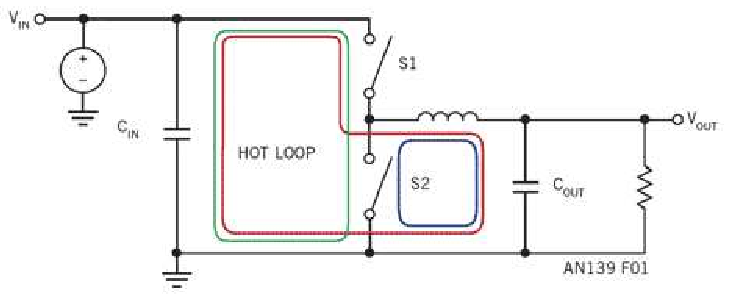
\includegraphics[scale=1]{pdf/outros/hotloop.pdf}
            	\label{fig:hot_loop_buck}
             	\indentedfont[12.5cm]{Adaptado de \citeonline{ref:EMC_HotLoop_kueck}}
            \end{figure}
            
            Quando a chave S1 está fechada, a corrente pulsada do circuito segue através do \textit{loop} vermelho. Quando a chave S2 está fechada, a corrente pulsada segue através do \textit{loop} azul. Porém, a área de \textit{hot loop} consiste na região em verde, onde flui uma corrente totalmente comutada, variando de zero a corrente de pico e de volta para zero. O mesmo ocorre em outros conversores \cite{ref:EMC_HotLoop_kueck}. 
            
            Dessa forma, \citeonline{ref:EMC_HotLoop_kueck} afirma que para reduzir EMI, deve-se reduzir a região na PCB do loop verde tanto quanto possível. Na qual, de uma perspectiva da EMI, \textit{hot loops} pequenos são os melhores.
            
            \citeonline{ref:EMC_artigo_Texas} ainda adverte que um bom \textit{layout} de PCB deve dispor os capacitores o mais próximo possível dos pinos de entrada e referência (tornando a área do \textit{loop} a menor possível). Portanto, a colocação dos capacitores de entrada deve ser uma das primeiras considerações, ao projetar qualquer conversor.
            
            %%%%%%%%%%%%%%%%%%%%%%%%%%%%%%%%%%%%%%%%%%%%%%%%%%%%%%%%%%%%%%%%%%%
            \subsubsection{Dissipadores} \label{cap:fund_emc_conv_mitig_dissip}
            %%%%%%%%%%%%%%%%%%%%%%%%%%%%%%%%%%%%%%%%%%%%%%%%%%%%%%%%%%%%%%%%%%%
            
            No estudo sobre o caminho pelo qual um ruído se propaga, é importante considerar a conexão do semicondutor com o seu dissipador, como mostrado na \autoref{fig:dissipador_semi}. Para \citeonline{ref:EMC_livro_PrintedCircuit}, os dissipadores de calor, por serem de metal e conterem estruturas de aletas, dependendo do harmônico produzido pelo semicondutor que estão conectados, suas dimensões o tornam eletricamente capazes de começar a irradiar energia eletromagnética. 
            
            \begin{figure}[H]
            	\centering
            	\caption{Conexão do dissipador ao semicondutor}
            	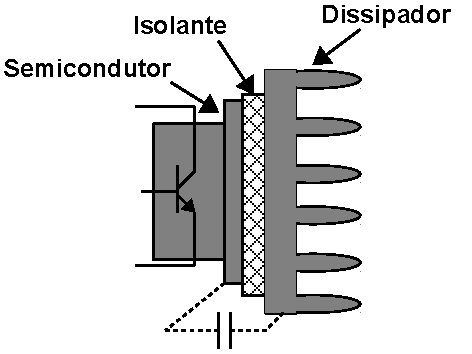
\includegraphics[scale=.8]{pdf/outros/dissipador.pdf}
            	\label{fig:dissipador_semi}
             	\indentedfont[7cm]{Adaptado de \citeonline{ref:EMC_phd_schlichting}}
            \end{figure}
            
            Dessa forma, \citeonline{ref:EMC_livro_PrintedCircuit} apresenta como uma possível técnica para redução da EMI a conexão dos dissipadores de calor na referência do circuito. Segundo o autor, usar um dissipador de calor conectado a referência cria um escudo de Faraday, evitando que a energia de alta frequência do semicondutor irradie para o espaço livre ou corrompa componentes adjacentes. 
            
            Ainda, um dissipador de calor conectado a referência, quando isolado, funciona como um grande capacitor de desacoplamento de modo comum entre o semicondutor e a referência. Este capacitor de modo comum é capaz de acoplar ou desviar a energia de alta frequência do dispositivo \cite{ref:EMC_livro_PrintedCircuit}.
            
            %%%%%%%%%%%%%%%%%%%%%%%%%%%%%%%%%%%%%%%%%%%%%%%%%%%%%%%%%%%%%%%%%%%
            \subsubsection{Capacitores} \label{cap:fund_emc_conv_mitig_cap}
            %%%%%%%%%%%%%%%%%%%%%%%%%%%%%%%%%%%%%%%%%%%%%%%%%%%%%%%%%%%%%%%%%%%
            
            \citeonline{ref:EMC_livro_Paul} afirma que os capacitores são geralmente a escolha mais comum como elemento supressor de ruído, uma vez que são de fácil instalação em um produto já montado, fornecendo um caminho de baixa impedância para as altas frequências. Porém o mesmo ainda ressalta que há erros frequentes na escolha e eficácia dos capacitores utilizados. 
            
            Para \citeonline{ref:EMC_livro_NoiseReduct}, a frequência de operação de um capacitor é uma das considerações mais importantes. A relação entre capacitância e volume em um capacitor eletrolítico, por exemplo, é maior do que para qualquer outro tipo de capacitor, porém, um capacitor eletrolítico de alumínio pode ter uma \abreviatura&{ESR}{equivalent series resistance}{resistência série equivalente} de até 1 $\Omega$, ou até superior em alguns casos.
            
            A frequência máxima de uso para um capacitor é geralmente limitada pela indutância L da estrutura do capacitor, proveniente de seus terminais. Abaixo da frequência de auto-ressonância do capacitor, o mesmo tem comportamento capacitivo e uma impedância que diminui com a frequência. Porém, acima dessa frequência, o capacitor parece indutivo e tem uma impedância que aumenta com a frequência. Sendo, portanto, capacitores recomendados para frequências menores e normalmente não recomendados em frequências muito elevadas. A \autoref{fig:cap_equiv} apresenta o circuito equivalente de um capacitor \cite{ref:EMC_livro_NoiseReduct}. 
            
            \begin{figure}[H]
            	\centering
            	\caption{Circuito equivalente de um capacitor}
            	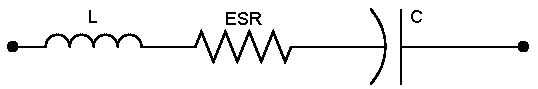
\includegraphics[scale=.8]{pdf/outros/cap_equiv3.pdf}
            	\label{fig:cap_equiv}
             	\indentedfont[8cm]{Adaptado de \citeonline[p.~194]{ref:EMC_livro_NoiseReduct}}
            \end{figure}
            
            Dessa forma, \citeonline{ref:EMC_livro_NoiseReduct} adverte que, para uso em frequências mais altas, deve-se optar por capacitores com valores de ESR e indutância mais baixas.
            
            %%%%%%%%%%%%%%%%%%%%%%%%%%%%%%%%%%%%%%%%%%%%%%%%%%%%%%%%%%%%%%%%%%%
            \subsubsection{Posicionamento dos elementos magnéticos} \label{cap:fund_emc_conv_mitig_magn}
            %%%%%%%%%%%%%%%%%%%%%%%%%%%%%%%%%%%%%%%%%%%%%%%%%%%%%%%%%%%%%%%%%%%
            % Interferência entre indutores [Schlichting]
            
            O posicionamento dos elementos magnéticos também é importante. Segundo \citeonline{ref:EMC_phd_schlichting}, os elementos magnéticos do circuito, por serem elementos que facilitam a propagação de campos, necessitam de certa atenção ao serem colocados, buscando uma posição na qual seus campos induzam o mínimo de tensão e corrente em outros elementos do circuito. \citeonline{ref:EMC_joabel_aula6} complementa que deve-se evitar a proximidade de dois elementos magnéticos (indutores e/ou transformadores) que operem em alta frequência, devido ao fluxo magnético. 
            
            Ainda, segundo \citeonline{ref:EMC_livro_Paul}, os elementos ferromagnéticos têm um efeito considerável na emissão irradiada, uma vez que, se mal projetados, parte do fluxo magnético presente nos mesmos dispersa e completa o caminho magnético através do ar circundante, como apresentado na \autoref{fig:entreferro}.
            Dessa forma, \citeonline{ref:EMC_phd_schlichting} adverte que, sempre que possível, deve-se utilizar toroides ou núcleos com entreferro reduzido a fim de evitar fluxo disperso. 
            
            \begin{figure}[H]
            	\centering
            	\caption{Fluxo magnético disperso em um elemento magnético com entreferro}
            	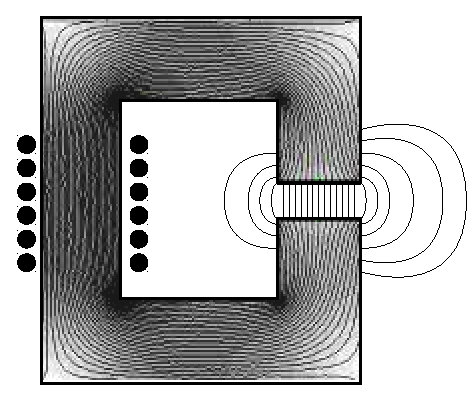
\includegraphics[scale=.8]{pdf/outros/entreferro.pdf}
            	\label{fig:entreferro}
             	\indentedfont[7cm]{Elaboração própria (2021)}
            \end{figure}
            
            %%%%%%%%%%%%%%%%%%%%%%%%%%%%%%%%%%%%%%%%%%%%%%%%%%%%%%%%%%%%%%%%%%%
            \subsubsection{Núcleo de ferrite} \label{cap:fund_emc_conv_mitig_choke}
            %%%%%%%%%%%%%%%%%%%%%%%%%%%%%%%%%%%%%%%%%%%%%%%%%%%%%%%%%%%%%%%%%%%
            % Uso de indutores choke para confinar ruído [montrose]
            
            Segundo \citeonline{ref:EMC_livro_PrintedCircuit}, o uso de dispositivos de ferrite (como toroides, núcleos, \textit{beads} e outros) são largamente utilizados na atenuação de sinais de frequências maiores que centenas de quilohertz. 
            
            Para \citeonline{ref:EMC_livro_PrintedCircuit} há três usos comuns de dispositivos de ferrite, sendo eles:  
            
            \begin{alineas}
                \item o uso como blindagem, na qual o dispositivo de ferrite isola condutores, componentes ou circuitos de campos eletromagnéticos dispersos;
                
                \item o uso do ferrite junto a um capacitor, na qual é criado um filtro passa-baixa que é indutivo-capacitivo em frequências baixas e dissipativo em frequências mais altas;
                
                \item o uso como elemento dissipativo, na qual o ferrite remove ou absorve a energia eletromagnética presente em uma linha de transmissão e dissipa essa alta frequência como calor. Isso se dá devido ao material de ferrite evitar oscilações parasitas ou atenuar o acoplamento de sinais indesejados que viajam ao longo de terminais de componentes, fios de interconexão, trilhas ou cabos. 
            \end{alineas}
            
            Para as duas ultimas aplicações, o núcleo de ferrite suprime a EMI reduzindo as correntes de alta frequência que são emitidas de uma determinada fonte de ruído. Idealmente, ao ser introduzido no circuito, o ferrite resulta em uma alta impedância para correntes de alta frequência e uma impedância nula para as demais frequências \cite{ref:EMC_livro_PrintedCircuit}. 
            
            A forma mais comum de um dispositivos de ferrite é um \textit{bead}, conforme mostrado na \autoref{fig:bead_equiv}, na qual o material de ferrite é colocado em torno de um condutor. Assim, configurando uma impedância de alta frequência em série com o mesmo \cite{ref:EMC_livro_Paul}.
            
            \begin{figure}[H]
            	\centering
            	\caption{Circuito equivalente de um ferrite \textit{bead} em um condutor}
            	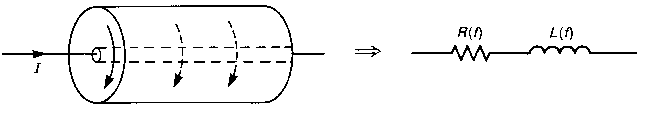
\includegraphics[scale=1]{pdf/outros/bead_equivalente.pdf}
            	\label{fig:bead_equiv}
             	\indentedfont[11cm]{\citeonline{ref:EMC_livro_Paul}}
            \end{figure}
            
            \citeonline{ref:EMC_livro_Paul} adverte que, devido à impedância do ferrite bead na faixa de frequência de sua eficácia ser limitada a várias centenas de ohms, são comumente usados em circuitos de baixa impedância, como fontes chaveadas. Não sendo diferente de outras aplicações de ferrite, pois são suscetíveis à saturação quando usados em circuitos que passam por correntes elevadas e frequência baixas.
            
            %%%%%%%%%%%%%%%%%%%%%%%%%%%%%%%%%%%%%%%%%%%%%%%%%%%%%%%%%%%%%%%%%%%
            \subsubsection{Frequência de chaveamento e tempo de comutação} \label{cap:fund_emc_conv_mitig_trans}
            %%%%%%%%%%%%%%%%%%%%%%%%%%%%%%%%%%%%%%%%%%%%%%%%%%%%%%%%%%%%%%%%%%%
            % Efeito da tensão, frequência e tempo de subida no gate do transistor [Schlichting, Daimer, Hegarty]
            
            Como já mencionado, do ponto de vista de potência, quanto menor o tempo de subida e descida da comutação dos semicondutores, menores serão as perdas de potência do circuito. Porém, transientes rápidos podem causar oscilações nos semicondutores (transistores e diodos), causando problemas de interferência eletromagnética \cite{ref:EMC_artigo_Texas}. 
            
            Segundo \citeonline{ref:EMC_artigo_Texas}, uma solução simples consiste em aumentar o valor do resistor em série com o terminal de Gate do transistor. O aumento desse valor de resistência aumentará o tempo de subida do sinal comutado, diminuindo a derivada de tensão e corrente do mesmo, o que pode diminuir a EMI às custas da eficiência energética.
            
            Para \citeonline{ref:EMC_phd_schlichting}, outra alternativa para redução da emissão conduzida, relacionada ao chaveamento dos semicondutores, trata-se da redução da frequência de chaveamento. Utilizando esta técnica, busca-se alocar a frequência fundamental do chaveamento o mais longe possível da faixa medida pelas normas de EMC \cite{ref:EMC_artigo_schlichting}. Essa alternativa, apesar de simples, torna-se muitas vezes inviável em projetos de fontes chaveadas, por acarretar em filtros de maior volume, como visto na \autoref{cap:fund_elp}.
            
            
\begin{comment}

    \section{Compatibilidade eletromagnética}
    \subsection{Medidas}
    
    \citeonline[p.~3, tradução nossa]{montrose2000printed}
    
    \SI{120}{dB$\mu$\volt}
    
    \begin{citacao}
        \begin{alineas}[leftmargin=\leftskip+\labelwidth-\labelsep]
            \item Uma fonte geradora de energia;
            \item Um receptor que seja perturbado por essa energia quando a intensidade da interferência eletromagnética estiver acima de um limite tolerável;
            \item Um caminho de acoplamento entre a fonte e o receptor para a transferência de energia indesejada. \cite[p.~3, tradução nossa]{montrose2000printed}.
        \end{alineas}
    \end{citacao}
    
    \begin{figure}[H]
    	\centering
    	\caption{Interferência eletromagnética conduzida}
    	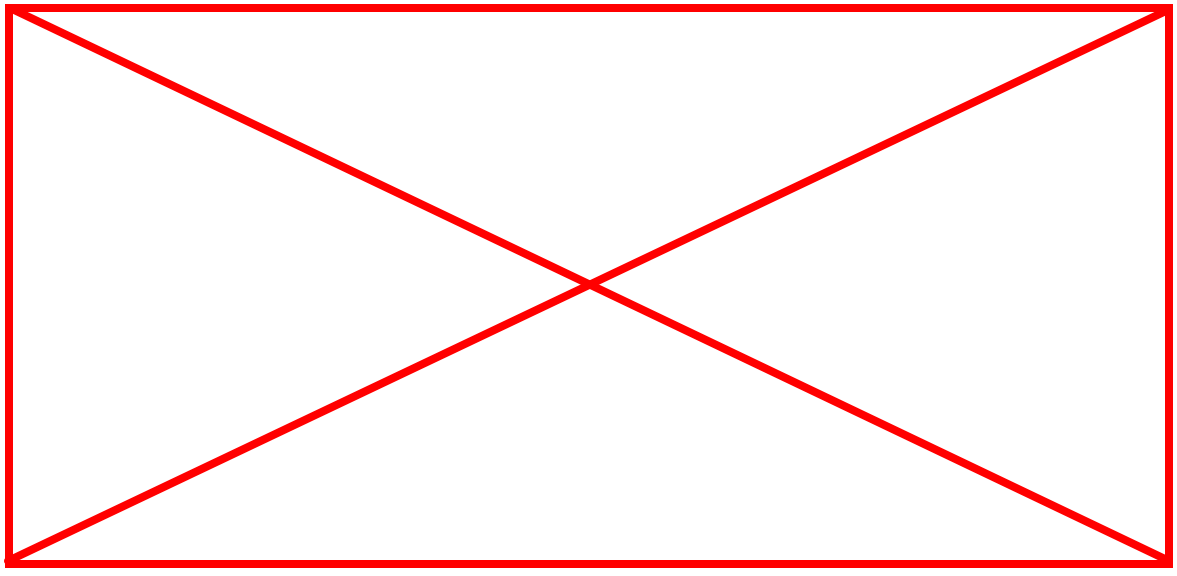
\includegraphics[scale=1.3]{noimage.png}
    	\label{fig:emi-conduzida}
     	\indentedfont[10cm]{Elaboração própria (2021)}
    \end{figure}
    
    \begin{equation} \label{eq:120dbuv}
        \text{Ganho} = 20\cdot \log_{10}\bigg(\frac{1V}{10^{-6}V}\bigg) = 120dB\mu V
    \end{equation}
    
    \begin{equation} \label{eq:buck_vo_Dvi}
        \begin{split}
            (\text{V}_\text{s} - \text{V}_\text{o})\cdot D\cdot T - \text{V}_\text{o}\cdot(T - D\cdot T) = 0 \\
            \text{V}_\text{o} &= \text{V}_\text{S}\cdot\text{D}
        \end{split}
    \end{equation}
    
    \begin{table}[H] %\ABNTEXfontereduzida
        \centering
        \caption{Lista de algumas normas da IEC referente a EMC}
        \label{tab:lista-normas}
        \begin{tabular}{|m{0.2\textwidth}|m{0.7\textwidth}|}
            \hline
            Norma           & Descrição \\
            \hline
            CISPR 16-x-x    & Especificação de equipamentos e métodos para medir emissão e imunidade\\
            \hline
            CISPR 11        & Equipamentos industriais, científicos e médicos - características das perturbações de radiofrequência - limites e métodos de medição \\
            \hline
        \end{tabular}
        \indentedfont[0.96\textwidth]{Elaboração própria (2021)}
    \end{table}

\end{comment}
